  \documentclass[10pt,conference,a4paper]{IEEEtran}
  \IEEEoverridecommandlockouts
  % ======================================================================
  %  CARBON: Gesture-Aware Multimodal Bug Reproduction for Android
  %  APSEC 2026 Technical Track
  %  Template: IEEE Conference (IEEEtran), 10 pages including references
  % ======================================================================
  \usepackage{cite}
  \usepackage{amsmath,amssymb,amsfonts}
  \usepackage{graphicx}
  \usepackage{xcolor}
  \usepackage{tikz}
  \usetikzlibrary{shapes.geometric,arrows.meta,positioning,calc}
  \usepackage{url}
  \usepackage{booktabs}
  \usepackage{multirow}
  \usepackage{array}
  \usepackage{stfloats}
  \usepackage{balance}
  \usepackage{hyperref}
  \hypersetup{hidelinks,pdfauthor={},pdftitle={},pdfsubject={},pdfkeywords={},pdfproducer={},pdfcreator={}}

  \newcommand{\YZ}[1]{{\color{blue} \sf (YZ: #1)}}

  % ======================================================================
  %  Anonymization toggle
  %  - For double-blind submission: leave \anonsubmissiontrue
  %  - For camera-ready:             set \anonsubmissionfalse
  % ======================================================================
  \newif\ifanonsubmission
  \anonsubmissiontrue   % <-- set to \anonsubmissionfalse after acceptance
  \newcommand{\repourl}{%
    \ifanonsubmission
      \url{https://github.com/bugfixops/CARBON}%
    \else
      \url{https://github.com/bugfixops/CARBON}%
    \fi}

  \begin{document}

  % ===================== TITLE & AUTHORS =====================
  \title{CARBON: Gesture-Aware Automated Reproduction of Android Bug Reports}

  % Double-blind: anonymous during submission, real identity on acceptance.
  % Author identity automatically switches based on the \ifanonsubmission toggle
  % in the preamble.
  \author{%
  \ifanonsubmission
    \IEEEauthorblockN{Anonymous Authors}
  \else
    \IEEEauthorblockN{Author Name(s) Omitted for Review}
    \IEEEauthorblockA{\textit{Affiliation omitted for review}\\
                      City, Country\\
                      email omitted for review}
  \fi
  }

  \maketitle

  % ===================== ABSTRACT =====================
  \begin{abstract}
  Reproducing bug reports is an essential but challenging task in mobile
  app maintenance. Recent LLM-driven tools mainly support basic UI actions,
  such as tapping and text input, but provide limited support for non-basic interactions, including scrolling and swiping. They also rely mostly on text-based UI representations, which
  may miss custom views and other elements not exposed in the view
  hierarchy. We study 3{,}629 Android bug reports and find that 13.0\% of
  reports requiring non-basic actions need complex or precision gestures
  that existing tools cannot express directly, such as pinch-to-zoom,
  drag-and-drop, and region/coordinate swipe. We investigate three baselines that provide partial support for
  some gesture actions but lack first-class support for complex gestures.
  To address this gap, we introduce \emph{CARBON}, an LLM-driven
  approach that combines a fourteen-action vocabulary, a
  multimodal prompt with an annotated screenshot and view hierarchy, and
  a dual oracle that verifies bug triggers using logcat and
  view-hierarchy state changes. On a gesture-diverse benchmark of 100 bug
  reports, CARBON achieves a bug reproduction rate of 88\%, substantially
  outperforming ReBL, the strongest baseline, which achieves 34\%.
  \end{abstract}

  \begin{IEEEkeywords}
  Android, bug reproduction, LLMs, test automation, gesture, multimodal
  \end{IEEEkeywords}

  % ===================== 1. INTRODUCTION =====================
  \section{Introduction}
  \label{sec:intro}

  In mobile development, reproducing user-submitted bug reports is a
  critical problem: developers must rebuild the UI states described in a
  report before identifying the root cause. However, such reports are
  often vague or incomplete~\cite{zimmermann,chaparro-s2r,rebl,adbgpt}.
  Unresolved bugs may also lead users to stop using the app~\cite{applause}.
  Thus, research has moved toward \emph{automated} bug-report
  reproduction, where a tool reads the report, drives the app, and
  confirms the symptom~\cite{recdroid,recdroidplus}. Recent LLM-driven tools (ReBL~\cite{rebl}, AdbGPT~\cite{adbgpt},
  ReActDroid~\cite{reactdroid}) show that LLMs~\cite{gpt4,gemini} can turn
  vague text into real UI events.
  Each tool employs an iterative LLM-driven process in which the model
  interprets the bug report, selects an action, observes the resulting
  state, and determines the next action. Building on prior work in
  crash replay~\cite{recdroid,recdroidplus,yakusu,crashtranslator,scopedroid}
  and LLM-based bug reproduction~\cite{libro}, these tools represent the
  current state of the art in automated bug reproduction. 

  However, existing tools, including ReBL, AdbGPT, and ReActDroid, still struggle to effectively reproduce bug reports due to three key limitations. First, they support only a narrow executable action vocabulary. ReBL lists seven
  UI actions, AdbGPT supports a similarly small set of five, and
  ReActDroid supports only click, text input, and long-press~\cite{rebl,adbgpt,reactdroid}
  (all listed in Table~\ref{tab:actions}). Yet all three lack first-class support for complex or precision gestures such as pinch-to-zoom, drag-and-drop,
  region/coordinate swipes, and timing-sensitive taps. Supporting such gestures is difficult: the tool must issue real multi-touch, timing, and coordinate-precise events that the app accepts as genuine, and aim them at on-screen targets that a text-only view hierarchy describes poorly. Second,
  they describe the UI as text only: when the
  view hierarchy is incomplete (for example, custom views that UIAutomator2
 cannot list), the LLM receives little actionable information even though
  the element is visible on screen. Third, existing tools often rely on the
  LLM to verify non-crash symptoms, leading to unsupported success claims.
  These limitations reduce accuracy for gesture, vision, and state-dependent
  bugs.
  
   To study whether these limitations matter at scale, we analyze 3,629 bug reports from 325 open-source Android projects. The reports are sampled in a gesture-neutral way using the GitHub \texttt{android} topic tag. After keyword matching and manual inspection, we find that \textbf{13.0\%} of reports requiring non-basic actions need complex or precision gestures that the baselines cannot express directly (full breakdown in Section~\ref{sec:prevalence}). These findings show that support for complex and precision gestures matters for effective bug reproduction, yet existing methods provide it inadequately.

  %To study whether these limits matter at scale, we study 2{,}582
  %bug reports from 229 open-source Android projects, sampled in a
  %gesture-neutral way through the GitHub \texttt{android} topic tag with
  %no app or gesture terms in the query (Section~\ref{sec:prevalence}).
  %After keyword matching and manual checking, we find that 7.6\% require
  %a simple gesture such as scrolling, swiping, or long-press, while 0.8\%
  %require a complex or precision gesture such as pinch-to-zoom,
  %drag-and-drop, or region/coordinate swipe.
  %The three baselines we study support simpler gestures only partially and lack first-class actions for the complex ones. Closing the gap needs three things: producing gestures the app's gesture detectors accept as real, reasoning about custom views, and checking non-crash symptoms without trusting the LLM.

To address these challenges, we introduce CARBON, an LLM-driven bug-reproduction tool designed for gesture-dependent Android bugs. CARBON operates through four main stages. First, it combines the UIAutomator2 view hierarchy with a screenshot containing numbered, color-coded widget annotations to provide structured and visual UI context. Second, the LLM returns one structured action or, for a transient-state interaction, a short action batch from a fourteen-action vocabulary covering basic UI actions, navigation/device actions, common gestures, and six complex or precision gestures. Third, CARBON translates the action or batch into ADB or UIAutomator2 commands and executes them on the device. Fourth, a dual oracle checks logcat and the view hierarchy to confirm the reported symptom. Using the updated UI state and execution feedback, the loop continues until the symptom is confirmed or the time budget expires.



\iffalse
  We introduce CARBON, an LLM-driven bug-reproduction tool that can support complex gesture: on Android, gestures and what is on the screen really
  matter. CARBON makes three design choices. First, it \emph{shows the
  LLM the screen}: each prompt pairs the UIAutomator2 view hierarchy with
  an annotated screenshot (numbered, color-coded boxes on every widget),
  so custom views and visual-only bugs become visible. Second, it
  \emph{acts with a fourteen-action vocabulary} that covers the gesture
  categories considered in our taxonomy, including pinch-to-zoom,
  drag-and-drop, region/coordinate swipe, and timing-sensitive
  taps. Third, it
  \emph{checks its own work} with a dual oracle: a logcat crash check
  plus a view-hierarchy state check (dialog text, disabled widgets,
  leftover text, and missing elements).
  

  These choices work together in a loop
  (Fig.~\ref{fig:overview}). At each step, CARBON reads and encodes the
  current screen, gives the LLM the bug report, lets it pick one action,
  runs that action on the device, and checks the result with the oracle.
  It repeats, recovering from failed steps through feedback until the
  oracle confirms the symptom or the time budget runs out, with no human
  help between turns.


  On a 100 bug gesture-diverse benchmark spanning eight gesture categories, CARBON
  reproduces \textbf{88 of 100 bugs}, compared to 34 for ReBL, 5 for
  ReActDroid, and 4 for AdbGPT once a uniform legitimacy audit is
  applied (54 of 100 self-reported); of the nine bugs ReBL reports as
  its own failures, CARBON reproduces seven, each addressing a
 weakness that ReBL itself names. Three ablations isolate each component: removing
  the overlay drops success to 61\%, removing the screenshot to 47\%
  (still above ReBL's 34\%), and disabling the oracle leaves 88\%
  self-reported but only 76\% once audited, a 12-point gap that measures
  false-positive prevention.
\fi

  On a 100-bug gesture-diverse benchmark covering eight non-basic action categories, CARBON reproduces \textbf{88 of 100 bugs}, compared with 34 for ReBL, 5 for ReActDroid, and 4 for AdbGPT after a uniform legitimacy audit (54 pre-audit tool-reported). On the nine bugs that ReBL reports as failures in its own benchmark, CARBON reproduces seven, each corresponding to a weakness identified by ReBL itself.
  
  In summary, this paper makes the following contributions:
  \begin{itemize}
  \item To our knowledge, CARBON is among the \emph{first} LLM-driven Android bug-reproduction approaches to explicitly support complex and precision-sensitive gestures through an extended fourteen-action vocabulary.
  \item Technically, CARBON pairs a multimodal prompt (annotated screenshot with the view hierarchy) with a dual logcat and state-change oracle, so it can both express gesture-dependent actions and verify non-crash symptoms without trusting the LLM's self-report.
  \item CARBON reproduces 88 of 100 gesture-diverse bugs, 54 percentage points above the strongest baseline (ReBL, 34/100), and reproduces seven of the nine bugs ReBL documents as failures.
  \item We release the implementation, benchmark, per-tool logs, and audit artifacts for future research~\cite{carbon}.
  \end{itemize}

  % ===================== 2. EMPIRICAL STUDY AND MOTIVATION =====================
  \section{Empirical Study and Motivation}
  \label{sec:motivation}

  In this section, we introduce the background for automated Android bug
  reproduction, present our empirical study of how often gestures are
  needed, and explain the challenges that shape CARBON's design.

  \subsection{Preliminaries}
  \label{sec:prelim}

  A \emph{UI widget} is a graphical element such as a button, text field, or image view, and a \emph{UI action} is an operation that a reproduction tool can execute on the app or device. We group UI actions into four families. \emph{Basic UI actions} are tap/click and text input, which all studied tools support~\cite{rebl,adbgpt,reactdroid}. \emph{Navigation/device actions}, such as \texttt{back} and device-orientation changes, are system-level operations rather than gestures. \emph{Gesture actions} go beyond tap and text and require movement, duration, timing, coordinate precision, or multi-touch input~\cite{androidmotion}; we split them into common gestures and complex or precision gestures. \emph{Common gestures} (scroll, swipe, long-press, and double-tap) are supported by at least one baseline in limited form. \emph{Complex or precision gestures} (pinch-to-zoom, drag-and-drop, region/coordinate swipe, timing-sensitive tap, picker-wheel scroll, and two-finger swipe) are the actions that the baselines cannot express directly~\cite{rebl,adbgpt,reactdroid}.
  A \emph{UI state} is the
  set of visible widgets and their attributes, read from the view
  hierarchy~\cite{androidmanual,uiautomator2}. Following ReBL~\cite{rebl},
  \emph{successful reproduction} means the buggy behavior is actually
  observed, not just that the action sequence finishes. We distinguish
  \emph{crash bugs} (a fatal exception or an Application Not Responding
  (ANR) error in logcat) from \emph{non-crash bugs} (a wrong or residual
  UI state) because the two demand different oracles: a crash is visible
  in logcat, whereas a non-crash symptom requires a state-level
  check~\cite{deepstate}. %a careful per-bug check labels 17 of our 100 benchmark bugs crash and 83 non-crash, with evidence in the replication package.

  \subsection{Empirical Study: How Often Gestures Are Needed in Practice}
  \label{sec:prevalence}

  To measure how often complex gestures matter in a natural bug stream, we
  assembled a gesture-neutral sample. Using the GitHub
  API~\cite{githubapi}, we discovered open-source Android projects through
  the \texttt{android} topic tag, with no app names or action terms in
  the query. From each project we collected issues carrying a bug label
  (open and closed, up to 15 per project). We did not filter by gesture
  content, so the sample reflects each project's general bug stream. This
  yielded 3{,}629 reports across 325 projects.

  We classify each report using the taxonomy in Section~\ref{sec:prelim},
  separating common gestures from complex or precision gestures. The categories
  are mutually exclusive: each report is counted once under the primary
  non-basic action that directly exposes the reported symptom; preceding or
  auxiliary actions are treated as setup.
  In all, 331 reports (9.1\%) require UI actions beyond basic tap or text
  input. A device-level orientation change, issued as a single command
  rather than a touch gesture, accounts for 63 of these (1.7\%). Gesture
  actions that at least one baseline supports in limited
  form appear in 225 reports (6.2\%): scroll (138 bugs, 3.8\%),
  swipe (55, 1.5\%), long-press (24, 0.7\%), and
  double-tap (8, 0.2\%). \textbf{\emph{Complex or precision gestures}},
  which the baselines cannot express directly, appear in 43 reports
  (\textbf{13.0\%} of the 331 non-basic-action reports; 1.2\% overall). Among these reports, 14 involve
  pinch-to-zoom (0.4\%), 12 drag-and-drop (0.3\%), and 8 region/coordinate
  swipe (0.2\%). Five involve timing-sensitive taps (0.1\%), two involve
  picker-wheel scrolling (0.1\%), and one involves a two-finger swipe
  (${<}0.1\%$). CARBON provides
  first-class support for six of these gestures: \texttt{pinch},
  \texttt{drag\_and\_drop}, \texttt{swipe\_region}, \texttt{quick\_tap},
  \texttt{picker\_scroll}, and \texttt{two\_finger\_swipe}, which
  together cover 42 of the 43 reports. The single remaining report
  requires a two-finger rotate, a gesture outside CARBON's vocabulary.

  Table~\ref{tab:actions} summarizes this difference: ReBL supports only
  a small subset of the actions needed for gesture-dependent reports,
  AdbGPT and ReActDroid support fewer actions, and CARBON adds six complex
  or precision gestures that the baselines cannot express directly. Many such reports depend on one precise action,
  such as dragging a seek bar, moving a map, or reordering a list item,
  that baselines can only approximate with a directional swipe.
  We treat double-tap as a common gesture and device-orientation as a
  navigation/device action: AdbGPT already supports a \texttt{double\_tap},
  and an orientation change is a single ADB command, so neither is unique
  to CARBON's action set. Section~\ref{sec:approach:actions} then details these six complex
  or precision gestures.

%  We checked these findings against three public datasets, AndroR2~\cite{andror2}, ReproBot~\cite{reprobot}, and the Android Functional Bugs Study~\cite{androidfunctionalbugs}; our inspection shows the same pattern: many unreproduced cases are limited by action coverage or oracle scope, not just by language understanding.

  \subsection{Motivation}
  \label{sec:comparison}

  Existing Android bug-reproduction tools (ReBL, AdbGPT, ReActDroid, and
  earlier non-LLM tools such as ReCDroid, Yakusu, CrashTranslator, and
  ScopeDroid) share one loop: read the report, choose a UI action
  against the current state, execute, observe, and iterate. Our
  study shows one shared limit: a narrow action vocabulary that omits the
  complex or precision gestures needed by 13.0\% of non-basic-action
  reports. Compared with prior tools, we identify two additional limitations: the need to reason about UI elements that are not fully captured by text-only view hierarchies, and the need to verify non-crash symptoms without relying solely on the LLM's self-report. These limits lead to the
  four challenges below, each addressed in Section~\ref{sec:approach}.

\begin{figure*}[!t]
  \centering
  \IfFileExists{motivation_example.png}{%
    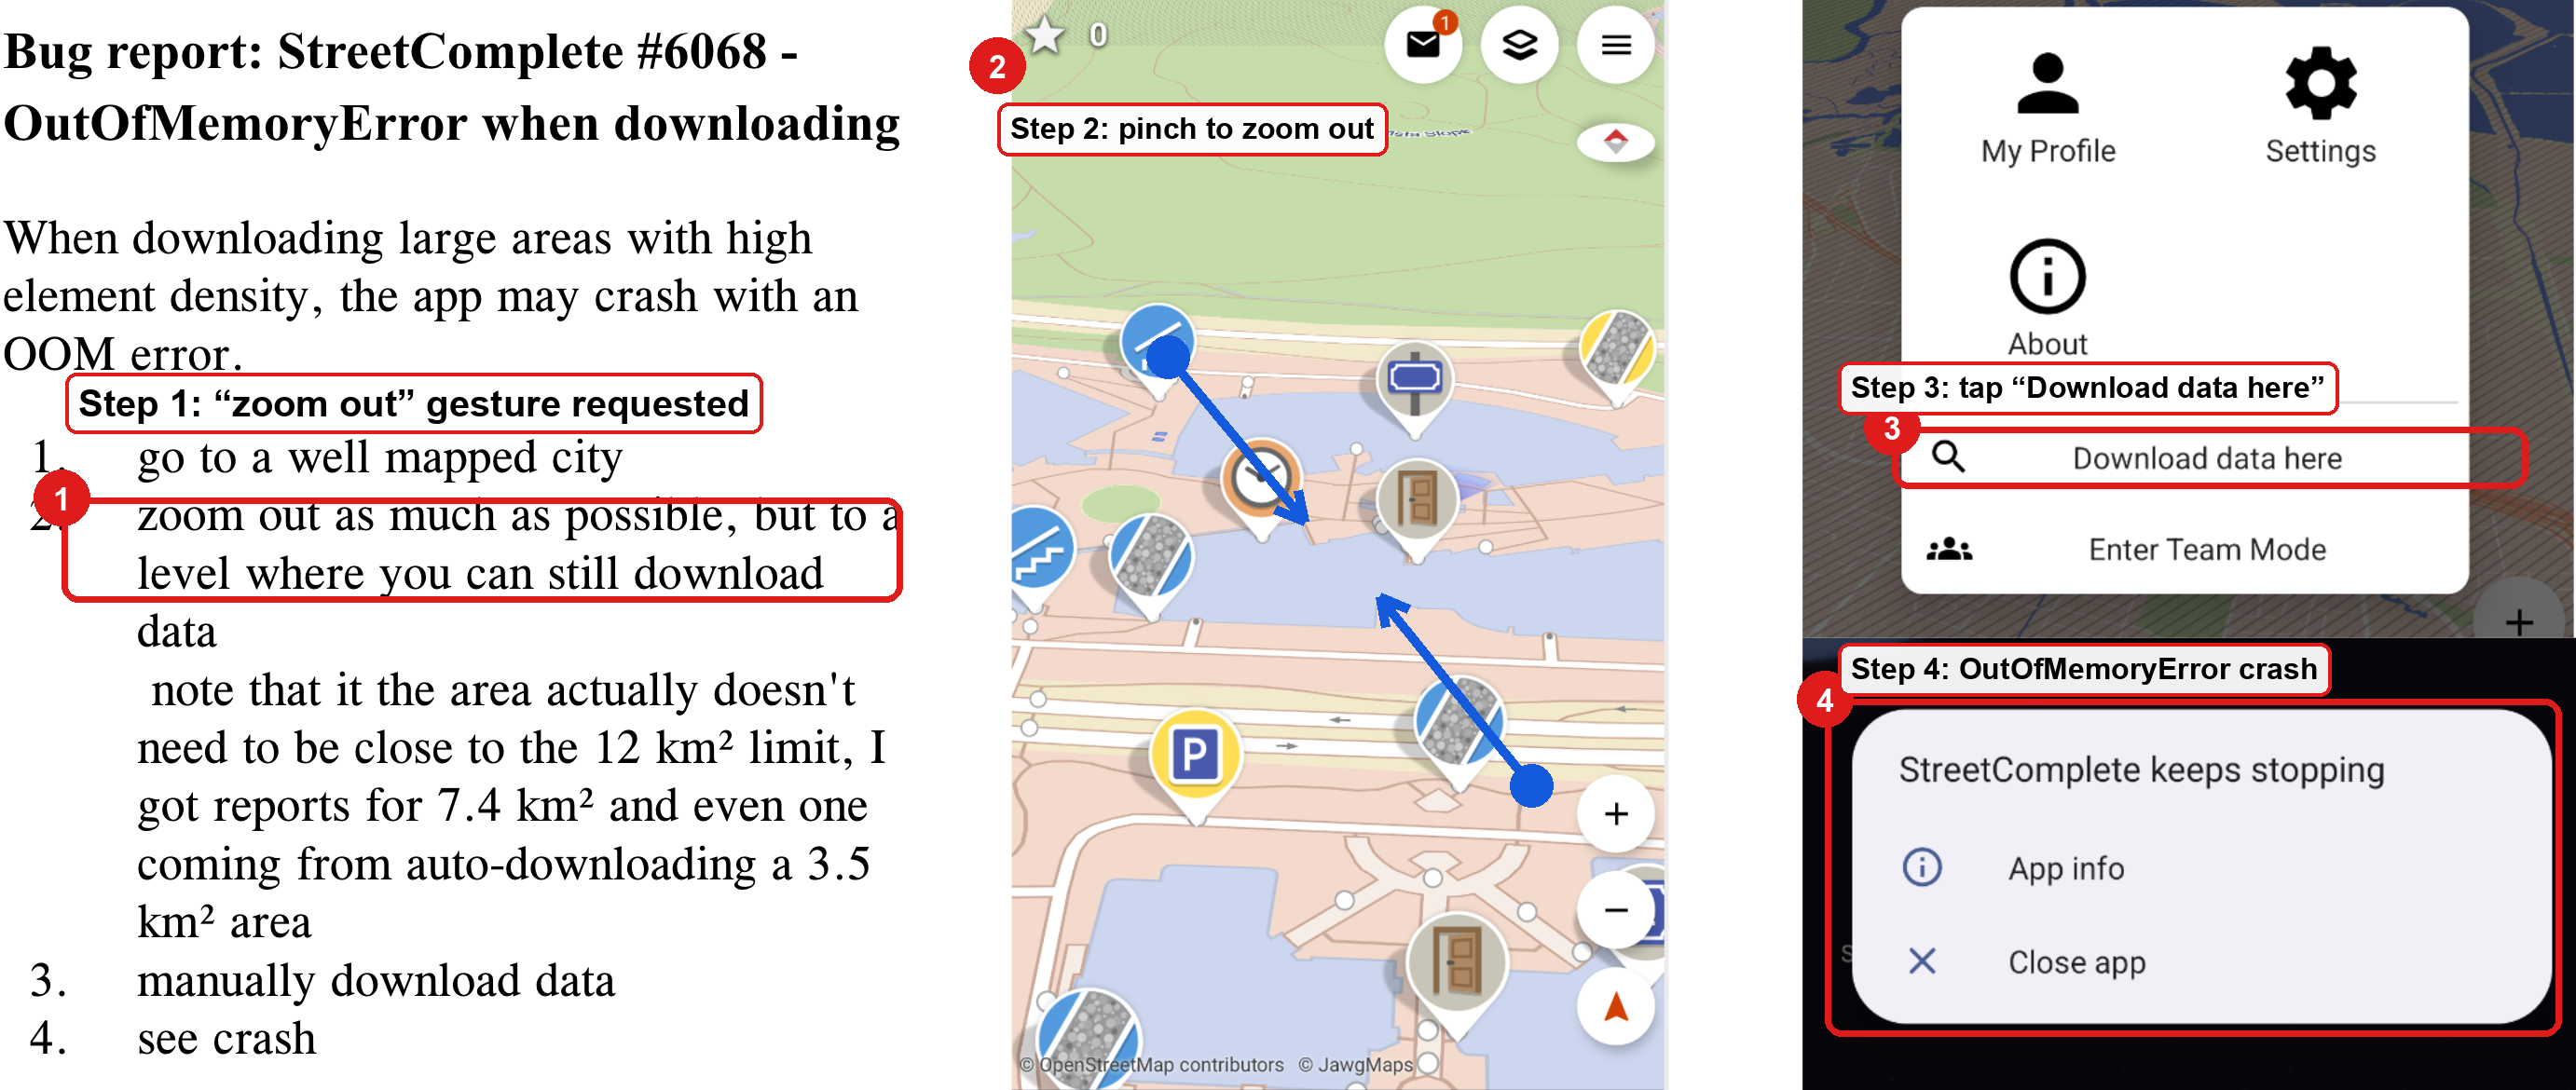
\includegraphics[width=\textwidth,keepaspectratio]{motivation_example.png}}{%
    \fbox{\parbox{0.96\textwidth}{\centering\vspace{1.6cm}\itshape Motivating figure to be added: StreetComplete\#6068.\vspace{1.6cm}}}}
  \caption{Motivating example: StreetComplete\#6068~\cite{streetcomplete6068}, whose crash requires a pinch-to-zoom on a map region that is under-specified by the view hierarchy.}
  \label{fig:motivating}
\end{figure*}

  \texttt{StreetComplete\#6068} serves as the
  running example (Fig.~\ref{fig:motivating}). In StreetComplete, users edit
  OpenStreetMap data on a full-screen map, and the bug requires them to
  zoom the map out over a dense area and then tap \emph{Download data
  here}, after which the app crashes with an \texttt{OutOfMemoryError}.
  This case is difficult for existing reproduction tools to handle,
  because the key action is not a tap or basic scroll but a real
  two-finger pinch-to-zoom on a map canvas. The crash is reached only by zooming the
  map out to a large area, so the buggy state is unreachable without the
  gesture, which the three baselines we study cannot express directly. The map is drawn as a
  canvas-like region under-specified by the view hierarchy, so a
  text-only representation
  gives the LLM little guidance about where to perform the gesture.
  CARBON reproduces the bug by grounding the map with the annotated
  screenshot, executing a \texttt{pinch} that none of the three baselines
  can perform, and confirming the crash with a logcat oracle.

  \paragraph*{Challenge 1: How to infer the complex gesture a bug report needs}
  Bug reports often describe actions in informal language, such as ``zoom in,'' ``drag it to the top,'' or ``tap when the dialog appears,'' without naming the exact executable action. The challenge is to map such ambiguous wording to the correct gesture; otherwise, the tool may execute a tap or scroll and fail to reach the buggy state. For example, in StreetComplete\#6068 (Fig.~\ref{fig:motivating}), ``zoom out as much as possible'' must be interpreted as pinch-to-zoom, not as a tap or basic scroll. CARBON addresses this challenge by giving the LLM the verbatim bug report together with explicit per-action use rules. At each step, it emits one typed action or, for a transient target, a short batch from the action vocabulary, resolving informal wording into concrete actions and parameters (Section~\ref{sec:approach:actions}).

  \paragraph*{Challenge 2: How to ground the gesture on the current screen}
Identifying the gesture type alone is insufficient; the tool must also determine its precise location. Android widgets interpret the same gesture differently depending on its start and end coordinates, path, duration, and touch points, so a gesture that lands off the target region fails to trigger the bug. Grounding is particularly difficult when the target is absent from the view hierarchy, as with a map canvas or picker dial. CARBON supports coordinate-aware action selection and execution by including explicit coordinate and timing parameters in each action. The LLM anchors the action to a widget using its legend index \texttt{\#k} or to raw screenshot coordinates when the target is absent from the hierarchy. The executor then translates the selected action into an on-device command (Sections~\ref{sec:approach:actions} and~\ref{sec:approach:execute}).

  \begin{table}[t]
  \caption{Action vocabularies of CARBON and the three baselines.}
  \label{tab:actions}
  \centering
  \scriptsize
  \setlength{\tabcolsep}{3pt}
  \renewcommand{\arraystretch}{1.2}
  \begin{tabular*}{\columnwidth}{@{\extracolsep{\fill}}llcccc@{}}
  \toprule
  \textbf{Family} & \textbf{Action} & \textbf{CARBON} & \textbf{ReBL} & \textbf{AdbGPT} & \textbf{ReActDroid} \\
  \midrule
  \multirow{2}{*}{Basic UI}
    & click               & \checkmark & \checkmark & \checkmark & \checkmark \\
    & set\_text           & \checkmark & \checkmark & \checkmark & \checkmark \\
  \midrule
  \multirow{2}{*}{Navigation/device}
    & back                & \checkmark & \checkmark &            &            \\
    & orientation         & \checkmark & \checkmark &            &            \\
  \midrule
  \multirow{4}{*}{\shortstack[l]{Common\\gesture}}
    & scroll              & \checkmark & \checkmark & \checkmark &            \\
    & swipe               & \checkmark & \checkmark &            &            \\
    & double\_tap         & \checkmark &            & \checkmark &            \\
    & long\_click         & \checkmark & \checkmark & \checkmark & \checkmark \\
  \midrule
  \multirow{6}{*}{\shortstack[l]{Complex/\\precision}}
    & pinch            & \checkmark &            &            &            \\
    & drag\_and\_drop   & \checkmark &            &            &            \\
    & swipe\_region     & \checkmark &            &            &            \\
    & quick\_tap        & \checkmark &            &            &            \\
    & picker\_scroll    & \checkmark &            &            &            \\
    & two\_finger\_swipe & \checkmark &            &            &            \\
  \midrule
  \textbf{Total} & & \textbf{14} & \textbf{7} & \textbf{5} & \textbf{3} \\
  \bottomrule
  \end{tabular*}

  \vspace{2pt}
  \raggedright\scriptsize
  Baseline columns are from each tool's published action
  table~\cite{rebl,adbgpt,reactdroid}. We treat
  \texttt{double\_tap} as a common gesture, not a complex one, since it is
  a standard two-tap interaction that AdbGPT also supports.
  \end{table}


  \paragraph*{Challenge 3: How to perceive UI targets that are under-specified by the text-only hierarchy}

The UIAutomator2 hierarchy provides useful textual UI information and can be directly included in the LLM prompt, but it is not sufficient for gesture-dependent bugs whose targets are defined visually. In StreetComplete\#6068, as shown in Fig.~\ref{fig:motivating}, the map region is visible on the screen, yet the hierarchy represents it only as a generic container, giving the LLM little guidance about where to perform the pinch-to-zoom. Thus, the tool must capture the screen image, process it into an LLM-readable representation, and help the LLM connect visual regions with executable actions. CARBON addresses this challenge by combining the view hierarchy with an annotated screenshot, where visible widgets and regions are marked with numbered, color-coded boxes (Section~\ref{sec:approach:capture}).
  
\iffalse  
Existing tools read the UI as text from the view hierarchy, so when it
  is incomplete (canvas-drawn custom views, picker dials, video overlays,
  accessibility widgets) the LLM gets little signal. StreetComplete's map
  is a clear case: it fills the screen but appears only as an empty
  container (Fig.~\ref{fig:motivating}). Even a complete hierarchy is
  lossy in each tool's encoding: ReBL collapses a 42-cell calendar into
  one scrollable handle~\cite{fossifycal1035}, ReActDroid exposes a flat
  three-verb list with no swipe, drag, or pinch, and AdbGPT matches only
  entities pre-extracted from the report, falling back to a
  \texttt{[MISSING]} tap~\cite{adbgpt}. CARBON instead exposes a flat
  numbered legend in which every visible widget is individually
  addressable (Section~\ref{sec:approach:capture}).

    Most LLM-driven tools decide success by asking the LLM whether the bug
  reproduced, which is risky: LLMs hallucinate, the oracle problem
  warns against letting the system under test judge
  itself~\cite{oracleproblem}, and
  even purpose-built multimodal LLM oracles reach only a 49\% detection
  rate~\cite{ollmandroid}. The verdict needs support from evidence
  outside the model, yet AdbGPT counts a fallback tap as a
  success~\cite{adbgpt} and ReBL takes non-crash verdicts from the LLM's
  reading of the screen (our audit overturns 16 of its 50 nominal
  successes, Section~\ref{sec:rq3}). CARBON adds a lightweight
  cross-check against logcat and the view hierarchy.
\fi

  \paragraph*{Challenge 4: How to verify a reproduction without trusting the LLM's self-report}

  Logcat can verify crashes, but non-crash symptoms such as incorrect
  dialogs or disabled widgets require UI-state evidence. Existing LLM-driven tools often rely on the LLM to determine whether such symptoms occurred, which can yield incorrect verdicts when the model hallucinates or misinterprets the screen. A reproduction verdict therefore needs evidence outside the model. CARBON addresses this challenge with a lightweight dual oracle that checks logcat for crash signals and the view hierarchy for state-level symptoms (Section~\ref{sec:approach:oracle}). We evaluate the oracle's contribution through the CARBON-NoOracle ablation (Section~\ref{sec:rq2}). In this independent run, 12 LLM-declared successes lack observable evidence. Comparison with the manual ground truth shows no false positives among the 88 confirmed successes and two cautious false negatives. These results appear in Section~\ref{sec:rq2} alongside the cross-tool legitimacy audit (Section~\ref{sec:rq3}, Reason~3).

  These challenges are interdependent: gesture support without visual
  grounding cannot reliably handle visually defined targets, while an
  oracle is useful only if the tool reaches the buggy state.

  % ===================== 3. CARBON APPROACH =====================
  \section{CARBON Approach}
  \label{sec:approach}

  CARBON runs in a four-stage loop (Fig.~\ref{fig:overview}): UI-state capture and encoding, LLM-based action selection, on-device action execution, and oracle-based verification. A termination controller ends the loop upon confirmed success, declared failure, or timeout. To capture the current app state, CARBON first obtains the device screenshot, XML view hierarchy, and execution feedback through UIAutomator2 and ADB. It then encodes the UI state using two complementary layers: an annotated screenshot with numbered, color-coded boxes on visible widgets, and a numbered element legend together with the view hierarchy. Given the bug report and the encoded UI state, the LLM returns one action or a short batch for a transient-state interaction, selected from the fourteen-action vocabulary. The executor translates the selected actions into concrete ADB or UIAutomator2 commands and runs them locally. After each action or batch, CARBON feeds the new UI state and execution feedback back to the LLM, forming an iterative reproduction loop. The loop terminates when the dual oracle confirms the reported symptom.

\iffalse
  CARBON reproduces a report by driving the device in a loop
  (Fig.~\ref{fig:overview}). At each step it reads the current screen
  and encodes it as a multimodal prompt (annotated screenshot, numbered
  legend, and view hierarchy), gives the LLM the verbatim bug report,
  and asks for one action from its fourteen-action vocabulary. It runs
  that action through ADB and UIAutomator2, then feeds the outcome and
  the new screen back. After each step a dual oracle checks whether the
  bug has triggered. The loop repeats until the oracle confirms the
  symptom, the LLM declares the bug unreproducible, or the time budget
  expires, with no human help between turns; the only manual work is
  preparing the bug-report text and the matching APK. We describe each
  step below.
  \fi

  \begin{figure}[!t]
      \centering
      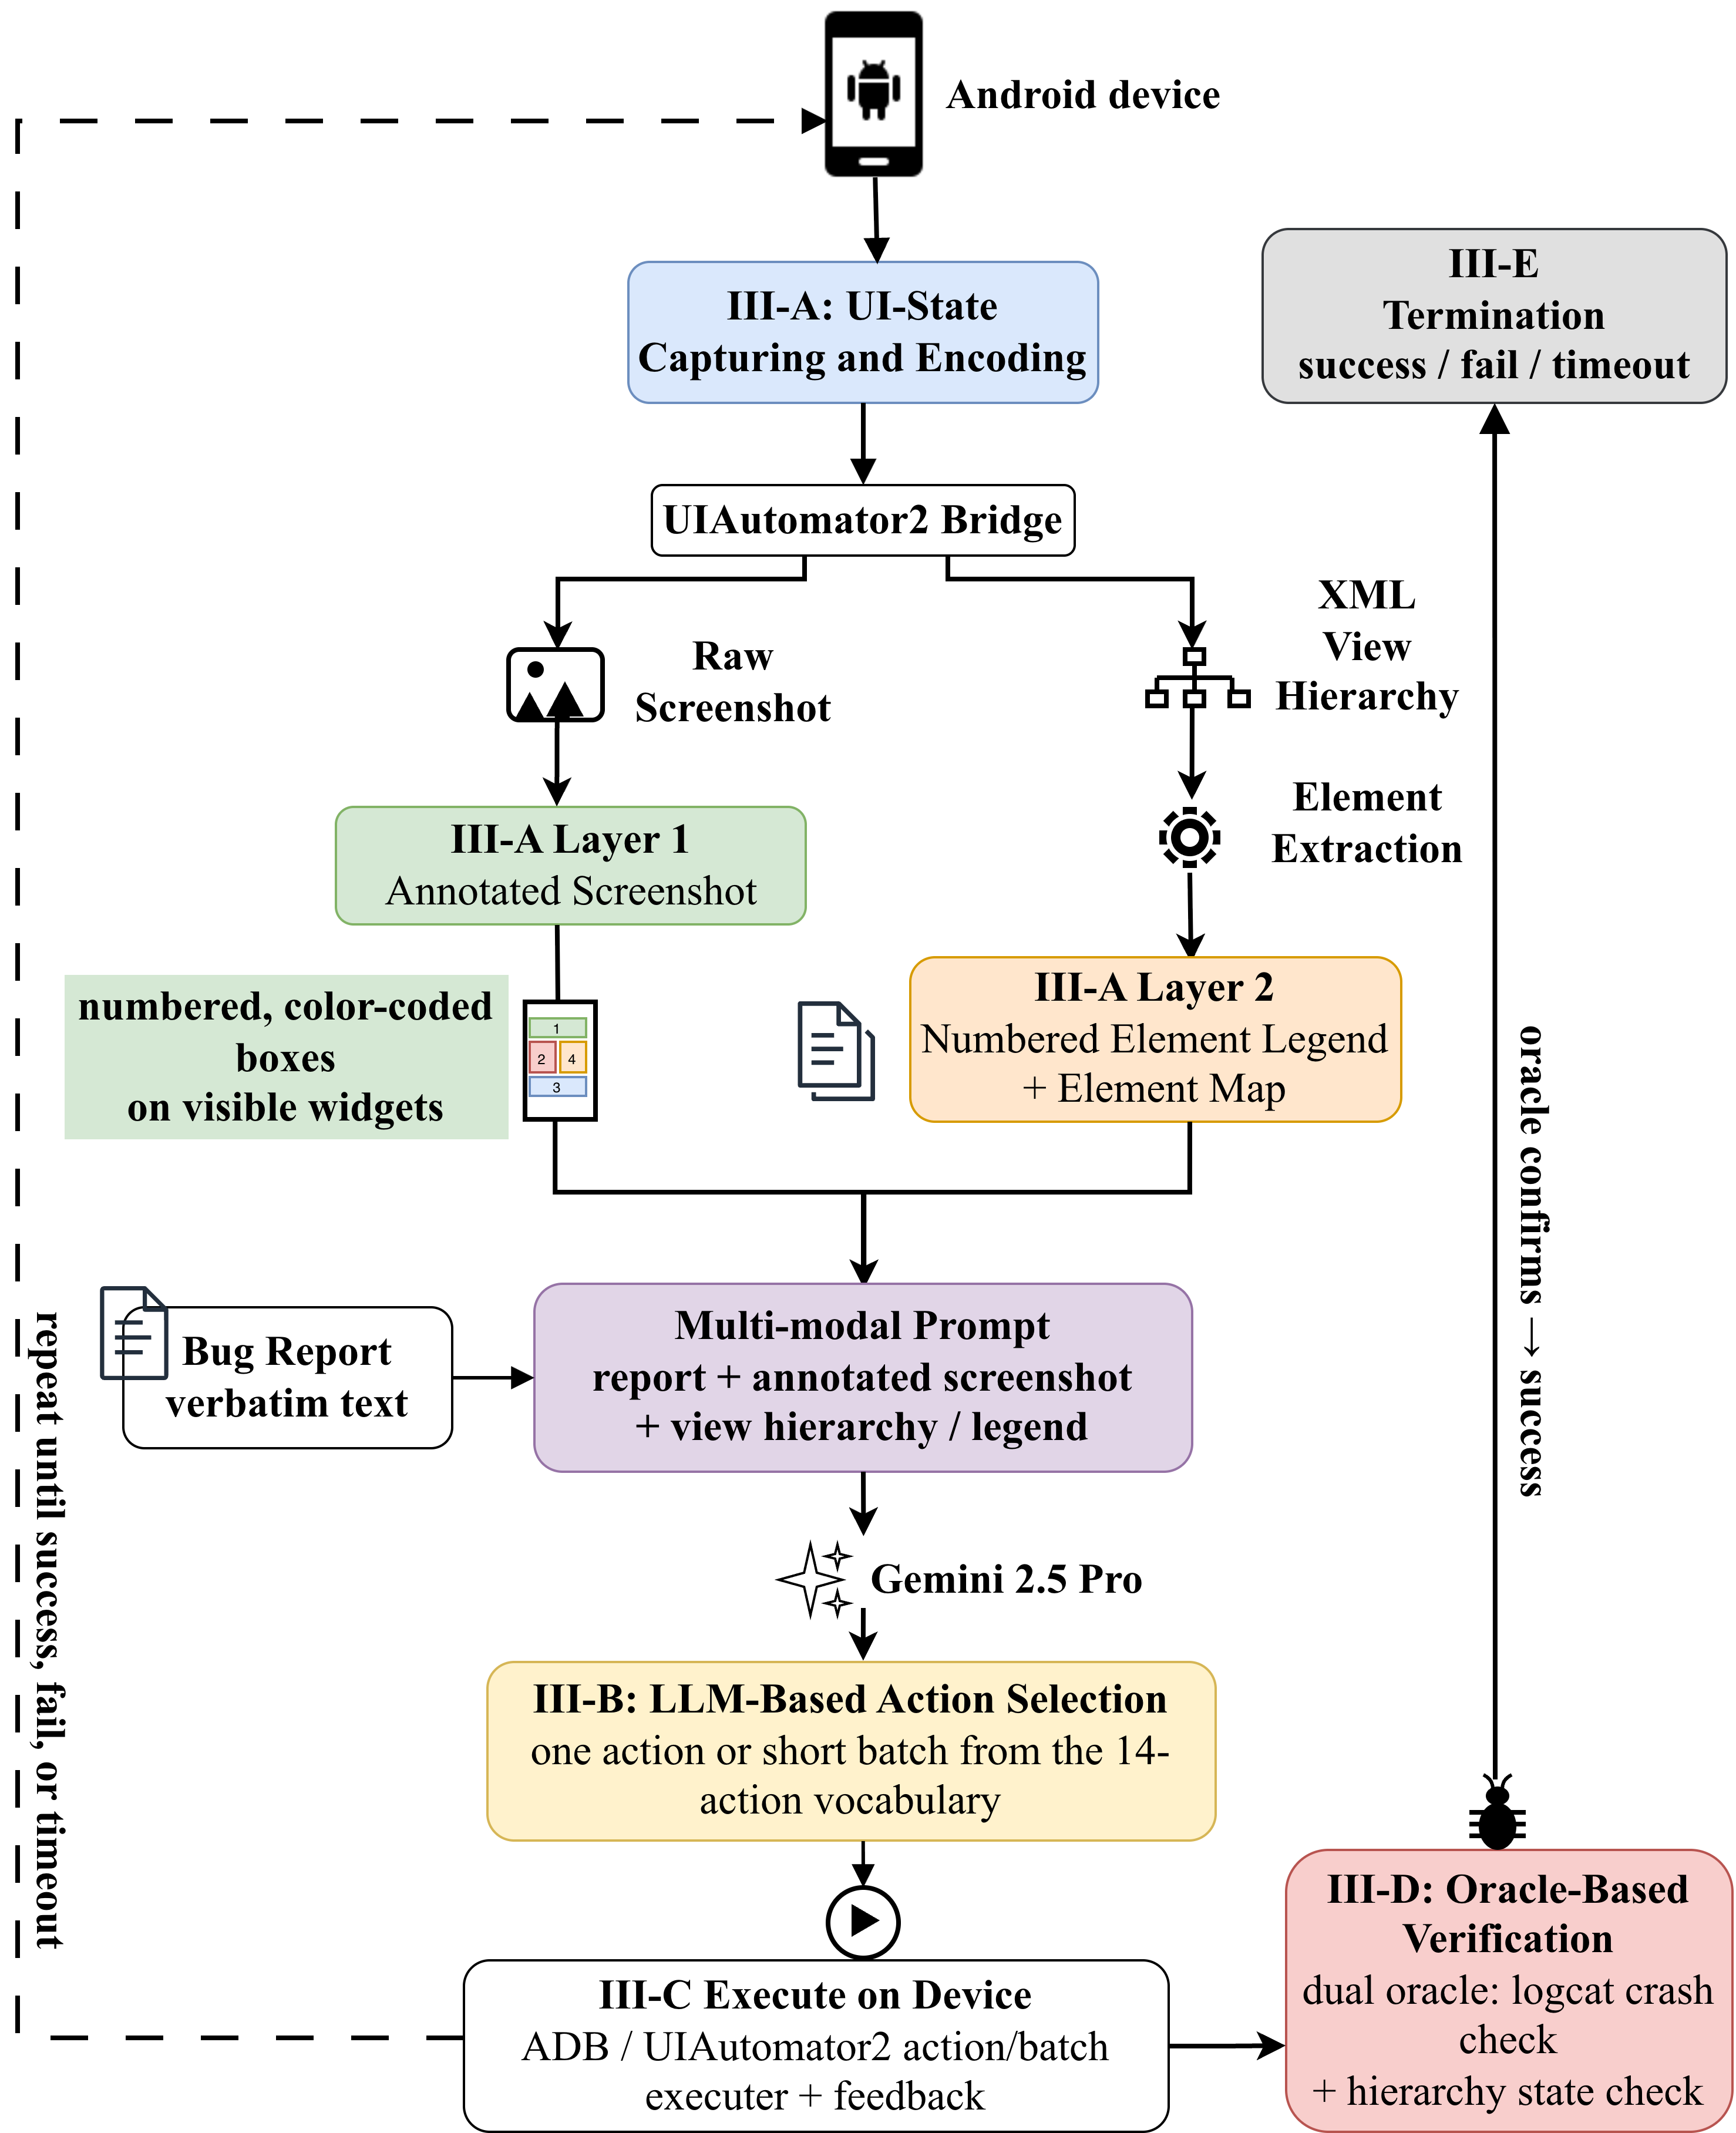
\includegraphics[width=\columnwidth,keepaspectratio]{architecture_diagram_paper.png}
      \caption{CARBON's reproduction loop.}
      \label{fig:overview}
  \end{figure}

  \subsection{Capturing and Encoding the UI State}
  \label{sec:approach:capture}

  At the start of every turn, CARBON queries the device through
  UIAutomator2~\cite{uiautomator2,androidmanual} for the screenshot and
  XML view hierarchy. Before each action or action batch, CARBON clears
  the logcat buffer and then captures new error-level entries produced during execution. It also records the
  foreground activity name, which the oracle uses to detect cases in which
  an app displays a recovery dialog instead of visibly crashing. From these, every
  prompt carries two UI encodings, shown in
  Fig.~\ref{fig:carbon-encoding} on the StreetComplete\#6068 map screen
  where the pinch-to-zoom precedes the download crash.

  \begin{figure}[!t]
      \centering
      \begin{minipage}[t]{0.50\columnwidth}
          \vspace{0pt}
          \centering
          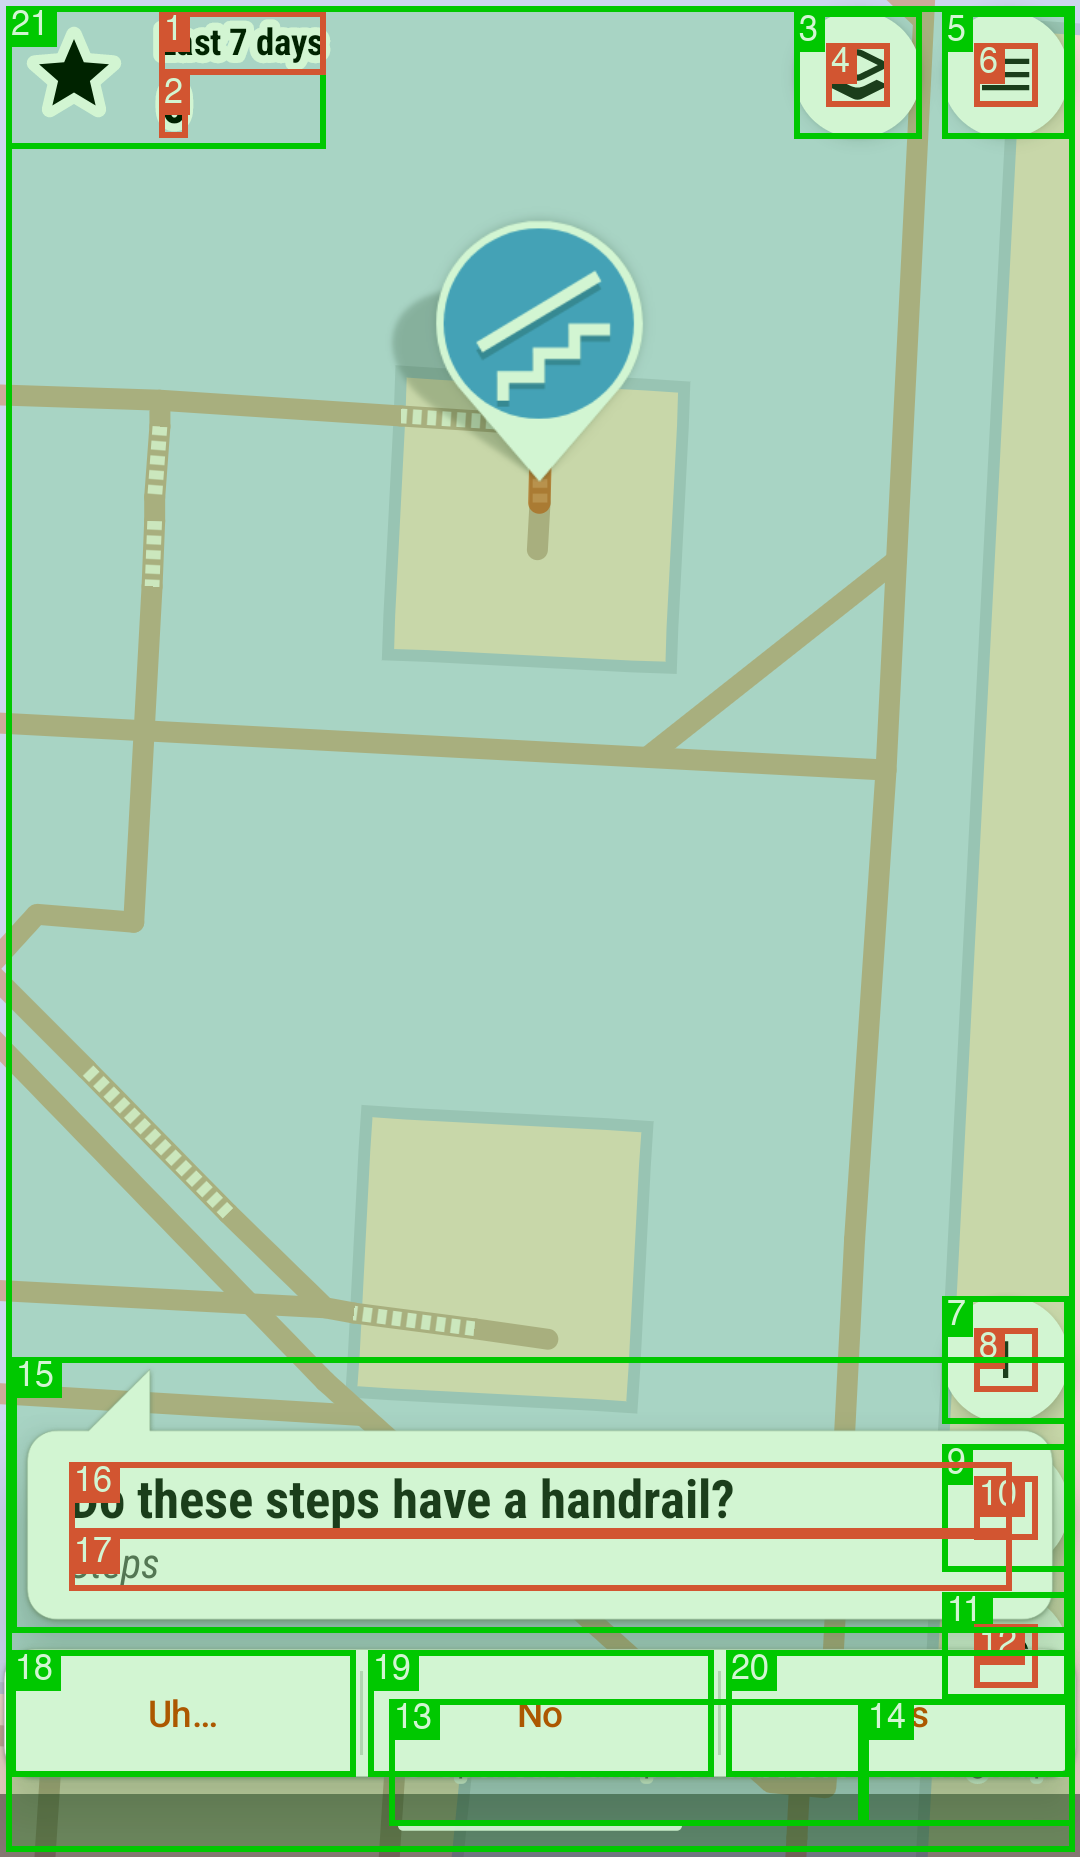
\includegraphics[width=\linewidth,keepaspectratio]{streetcomplete_map_annotated_full.png}
      \end{minipage}\hfill
      \begin{minipage}[t]{0.46\columnwidth}
          \vspace{0pt}
          \scriptsize
          \ttfamily
          \raggedright
          Element map: 22 elements\\
          GREEN [C]=clickable,\\
          RED [T]=text\\[2pt]
          \#1 \ [T] "Last 7 days" \mbox{[159,74][325,137]}\\
          \#4 \ [T] "Overlays" \mbox{[826,106][889,169]}\\
          \#6 \ [T] "Menu" \mbox{[974,106][1037,169]}\\
          \#8 \ [T] "Zoom in" \mbox{[974,1391][1037,1454]}\\
          \#10 [T] "Zoom out" \mbox{[974,1539][1037,1602]}\\
          \#12 [T] "Follow me" \mbox{[974,1687][1037,1750]}\\
          \#16 [T] "\ldots handrail?" \mbox{[69,1525][1011,1596]}\\
          \#17 [T] "Steps" \mbox{[69,1596][1011,1653]}\\
          \#18 [C] "Uh\ldots" \mbox{[10,1713][355,1839]}\\
          \#19 [C] "No" \mbox{[368,1713][713,1839]}\\
          \#20 [C] "Yes" \mbox{[726,1713][1070,1839]}\\
          \#21 [C] map \mbox{[0,0][1080,1920]}
      \end{minipage}

      \vspace{4pt}
      \makebox[0.50\columnwidth][c]{\footnotesize (a) Annotated screenshot}\hfill
      \makebox[0.46\columnwidth][c]{\footnotesize (b) Numbered element legend}
      \caption{Multimodal UI encoding of the StreetComplete\#6068 map screen.}
      \label{fig:carbon-encoding}
  \end{figure}

  \paragraph*{UI Encoding 1: annotated screenshot}

The annotated screenshot conveys the screen and the spatial location of UI targets. The XML hierarchy alone cannot capture this spatial information for custom views, map regions, picker dials, and other visually defined widgets. A raw screenshot also leaves target localization to the model; visual-grounding work addresses this challenge explicitly~\cite{cogagent,seeact}. CARBON removes zero-area, off-screen, or uninformative non-interactive hierarchy nodes. Nodes take the first matching class: focused, editable, scrollable, checkable, clickable, or text-bearing. \emph{Download data here} matches clickable and text-bearing; clickable comes first, so it receives that class. Using the Pillow imaging library~\cite{pillow}, it then overlays a numbered box colored by that class, such as green for clickable nodes and red for text-bearing nodes (Fig.~\ref{fig:carbon-encoding}). The shared index uniquely identifies each node across both representations. On the StreetComplete\#6068 map (Fig.~\ref{fig:carbon-encoding}a), the whole map is a single element (\#21) with no sub-target in the hierarchy. The annotation enables the LLM to ground the pinch-to-zoom gesture using the screenshot, while controls such as \emph{Menu} and \emph{Overlays} remain individually targetable.

  \paragraph*{UI encoding 2: textual view hierarchy and numbered element legend}
The textual view hierarchy supplies attributes that pixels cannot recover, including exact bounds, content descriptions, resource identifiers, displayed text, and enabled or checked state. CARBON renders these attributes in a numbered legend that reuses the screenshot's indices, so a reference such as ``\#21'' points to the same node in both encodings (Fig.~\ref{fig:carbon-encoding}b). These attributes also drive oracle-based verification: a \texttt{DISABLED} spinner (\texttt{FieldBook\#137}~\cite{fieldbook137}) or residual \texttt{text="Joh"} (\texttt{Qksms\#1155}~\cite{qksms1155}) is a hierarchy check, not a vision one. CARBON also appends a per-region color summary and a step-to-step UI difference to surface visual-only changes such as theme glitches or wrong album art.

  \iffalse
  Many bugs live on widgets it
  never reports (canvas custom views, picker dials, video overlays,
  accessibility widgets), so a text-only tool is blind to them
  (Challenge~3). A raw screenshot is not enough either: vision-language
  models such as Gemini~2.5~Pro~\cite{gemini25pro} and GPT-4V~\cite{gpt4v}
  locate targets far more reliably when the prompt points at them than
  when they must find them in raw pixels~\cite{cogagent,seeact}. CARBON
  therefore overlays a numbered, color-coded box on every interactive
  widget (green clickable, orange editable, blue scrollable, purple
  checkable). It builds the overlay from the captured artifacts: it
  parses the UIAutomator2 hierarchy, drops zero-area, off-screen, and
  non-interactive nodes, classifies each survivor by a priority rule
  (focused, editable, scrollable, checkable, clickable, then
  text-bearing) that fixes its color, and draws the box with an index
  badge reused in the Layer~2 legend, so one number names one node in
  both views. On the StreetComplete\#6068 menu
  (Fig.~\ref{fig:carbon-encoding}a) each option, including
  \emph{Download data here}, becomes an individually targetable box; on
  the preceding map screen the same overlay grounds the pinch-to-zoom
  region that the hierarchy exposes only as an empty container, the kind
  of custom view UIAutomator2 ``fails to extract from the
  hierarchy''~\cite{rebl}.


  \paragraph*{UI encoding 2: textual view hierarchy and numbered element legend}
  The screenshot shows \emph{where} a widget is; the hierarchy says
  \emph{what} it is. CARBON sends the XML hierarchy as a numbered legend
  reusing the same indices (Fig.~\ref{fig:carbon-encoding}b), so a
  reference such as ``\#13'' resolves to one node. The hierarchy keeps the
  exact bounds, content descriptions, identifiers, text, and
  enabled/checked attributes that pixels cannot recover, which is what
  non-crash oracles need: spotting a \texttt{DISABLED} spinner
  (\texttt{FieldBook\#137}~\cite{fieldbook137}) or a residual
  \texttt{text="Joh"} (\texttt{Qksms\#1155}~\cite{qksms1155}) is a
  hierarchy check, not a vision one. CARBON also appends a per-region
  color summary and a step-to-step diff to help the LLM catch
  visual-only changes such as theme glitches or wrong album art; the
  screenshot ablation (Section~\ref{sec:rq2}) covers this indirectly.
  The gain is measurable: from the same UIAutomator2 hierarchy, CARBON's
  legend exposes a median of 23 addressable widgets per step (mean 31;
  90th percentile 58, over 1{,}334 logged steps), against a median of 4
  for ReBL and 6 for ReActDroid; AdbGPT encodes the hierarchy as HTML
  with per-element ids, a different format we do not score on this
  scale. The difference reflects encoding, not the platform.

\fi
  \subsection{Understanding the Bug Report and Selecting an Action}
  \label{sec:approach:actions}

   Along with the encoded UI state, CARBON feeds the verbatim bug report to the LLM and requires one executable action or, for a transient target, a short action batch in a predefined JSON format. As shown in Table~\ref{tab:instructions}, each prompt contains four blocks: the fixed task instruction, the bug report, the encoded UI state, and feedback from the previous step. Like ReBL~\cite{rebl}, CARBON does not extract S2R entities or normalize keywords; the LLM maps informal descriptions directly. The prompt pairs a fixed task instruction with per-action use rules, so the model emits valid, typed actions. The full template is in our replication package~\cite{carbon}. At each turn, the LLM returns a JSON list containing one action, a short action batch, or a result object. Batch actions run locally before the next UI capture or LLM call (see \texttt{quick\_tap} below). Each action object specifies its parameters, where a \texttt{\#k} target refers to the corresponding legend index in Fig.~\ref{fig:carbon-encoding}.



  \begin{table}[t]
  \caption{CARBON's instruction prompt.}
  \label{tab:instructions}
  \centering
  \footnotesize
  \renewcommand{\arraystretch}{1.3}
  \begin{tabular}{@{}p{0.17\columnwidth}p{0.74\columnwidth}@{}}
  \toprule
  \textbf{Component} & \textbf{Details} \\
  \midrule
  $\langle$Objective$\rangle$ &
  Reproduce an Android bug report: not only follow the steps to where the
  bug occurs, but confirm with external evidence that the buggy behavior
  is actually triggered. \\
  $\langle$Workflow$\rangle$ &
  We provide the app name, the verbatim bug report, and the current UI
  state (annotated screenshot, numbered legend, view hierarchy). You
  reply with one action or a short batch for a transient target; we
  execute it and return the outcome and new state. The loop continues
  until the dual oracle confirms the symptom or reproduction is declared
  failed. \\
  $\langle$Explanation$\rangle$ &
  (1)~Available actions: the fourteen-action vocabulary
  (Table~\ref{tab:actions}), addressed by legend index;
  (2)~response format: a JSON list of action objects or a result object;
  (3)~use-case rules, e.g.\ use \texttt{pinch} to zoom, start
  \texttt{drag\_and\_drop} from a handle, anchor targets not in the
  hierarchy using coordinates; (4)~termination: success when the oracle confirms the symptom, failure
  when the bug is judged unreproducible. \\
  \bottomrule
  \end{tabular}
  \end{table}

The vocabulary is derived from Android's input model~\cite{androidmotion} and the taxonomy of Section~\ref{sec:prelim}. It keeps the basic UI, navigation/device, and common-gesture actions the baselines already expose (in limited form; see Table~\ref{tab:actions}), and adds six complex or precision gestures. The LLM maps informal wording to a typed action (e.g., ``zoom out'' to \texttt{pinch}), and names its target by legend index \texttt{\#k} or by raw screenshot coordinates when it is not in the hierarchy. The parameters of each added action are described below.


  \emph{Pinch-to-zoom (\texttt{pinch}).} A pinch spreads or squeezes two
  fingers to zoom a view. CARBON's \texttt{pinch} issues a real
  two-pointer zoom that the app accepts as genuine. It takes a direction
  and an optional center \texttt{(cx,cy)} so it lands on the right widget.
  It reproduces StreetComplete\#6068~\cite{streetcomplete6068}, whose crash
  requires the map to be zoomed out.

  \emph{Drag-and-drop (\texttt{drag\_and\_drop}).} A drag-and-drop action presses
  an item and slides it from a start point to an end point, for example to
  reorder a list. CARBON's \texttt{drag\_and\_drop} first holds the handle
  for \texttt{hold\_ms}=800\,ms to enter drag mode, so the list does not
  switch into multi-select, as in Metrolist\#3227~\cite{metrolist3227}.

  \emph{Region/coordinate swipe (\texttt{swipe\_region}).}
  This action performs a swipe between two fixed coordinates. It is
  used when the target is not in the hierarchy, such as a custom canvas or
  picker dial, where a direction-only \texttt{swipe} would miss. CARBON
  uses this action to reproduce Fossify Gallery\#237~\cite{gallery237},
  whose bug report states that a vertical swipe on the right side of a
  video does not adjust the volume.

  \emph{Timing-sensitive tap (\texttt{quick\_tap}).} For transient-state
  bugs, CARBON can batch \texttt{quick\_tap} after another action, avoiding
  another UI capture or LLM call. After the preceding action's normal settle,
  it waits for \texttt{delay\_ms} (default 100\,ms), resolves the target in
  the updated UI or from coordinates, and taps once. A zero delay removes
  this added wait but not other latency. In AnkiDroid\#7138~\cite{anki7138},
  CARBON batched answer selection with \texttt{quick\_tap} on
  \emph{Show Answer}, using \texttt{delay\_ms}=0.

  \emph{Two-finger swipe (\texttt{two\_finger\_swipe}).} CARBON's
  \texttt{two\_finger\_swipe} moves two parallel pointers in one direction
  through UIAutomator2's native multi-touch. It reproduces
  Saber\#192~\cite{saber192}, where a two-finger pan on a zoomed
  note causes the pen tool to leave an unintended dot on the canvas.

  \emph{Picker-wheel scroll (\texttt{picker\_scroll}).} A date or time
  picker is a spinning \texttt{NumberPicker} dial that advances one value
  per short, slow drag, so an ordinary swipe overshoots or undershoots.
  Given the dial bounds and a tick count, CARBON's \texttt{picker\_scroll}
  issues short, tick-aligned drags that land on the chosen value. CARBON
  uses this action on the date picker in
  Memento\#169~\cite{memento169}.

  \subsection{Executing Actions and Feedback}
  \label{sec:approach:execute}

  Each action has an executor that translates its JSON object into an ADB
  or UIAutomator2 call; for example, \texttt{click} becomes a coordinate
  tap, while \texttt{pinch} issues a two-pointer gesture. For a batch,
  CARBON runs the actions consecutively before the next UI capture or LLM
  call and records each outcome separately. Failed or unparseable actions
  return feedback, and repeated subsequences trigger a loop warning. The
  next iteration captures the updated UI and continues until termination
  or the wall-clock budget expires.
 

  \subsection{Verifying the Symptom}
  \label{sec:approach:oracle}

  CARBON re-checks every self-declared success with two low-overhead,
  repeatable signals. The \emph{crash oracle} runs automatically: it scans
  error-level \texttt{adb logcat} for \texttt{FATAL EXCEPTION}, \texttt{ANR},
  and package-filtered exceptions, and it identifies crash-report dialogs.
  Non-crash bugs may leave no reliable logcat trace, so the \emph{state-change oracle}
  re-reads the post-action hierarchy for general anomalies: error or toast
  text, an unexpected disabled state (\texttt{FieldBook\#137}~\cite{fieldbook137}), leftover
  text (\texttt{Qksms\#1155}~\cite{qksms1155}), or a missing element
  (\texttt{KISS\#1481}~\cite{kiss1481}). Each non-crash success is then
  confirmed under the legitimacy audit (Section~\ref{sec:rq3}, Reason~3),
  and one without such evidence is not counted. %Because neither check accepts LLM self-report alone (Challenge~4), the oracle catches successes the LLM would otherwise claim falsely (the RQ2 CARBON-NoOracle ablation, Section~\ref{sec:rq2}, flips 12 such bugs).

  \subsection{Termination}
  \label{sec:approach:termination}

  A run ends in success when the oracle confirms the reported symptom. For crash bugs, this confirmation comes from the crash oracle; for non-crash bugs, the state-change oracle must corroborate the LLM's verdict, so a self-declared success without supporting evidence is not accepted. If the symptom is not confirmed, the run ends when the 1{,}800-second wall-clock budget expires or when the LLM declares the bug unreproducible. Unparseable outputs, failed actions, and detected repeated action patterns do not directly terminate the run; instead, they are returned as feedback and the loop continues. For example, in \texttt{FieldBook\#137} the LLM declared success, but the run ended as a confirmed reproduction only after the state-change oracle verified the \texttt{DISABLED} spinner in the post-action hierarchy (Section~\ref{sec:rq3}).
\iffalse
  A run ends in success when the oracle confirms the symptom (for crash
  bugs via a \texttt{check crash} action, for non-crash bugs when the
  state-change oracle corroborates the LLM's verdict, so a self-declared
  success with no signal does not stand), and otherwise when the
  1{,}800-second wall-clock budget expires or the LLM declares the bug
  unreproducible; unparseable output, dead actions, and detected repeats
  only inject feedback and continue, making the budget the binding stop
  for hard cases. Because the oracle underlies every reported number,
  we manually checked each of the 88 successes against its log and final
  screen, using the six criteria of Section~\ref{sec:rq3}. Two runs whose only symptom was a brief animation
  (\texttt{File-Manager\#195}~\cite{filemanager195},
  \texttt{LibreTube\#8245}~\cite{libretube8245}) were reclassified as
  failures, since the oracle cannot see animation. The auditor scripts
  and all per-bug logs are released.
  \fi

  % ===================== 4. EMPIRICAL STUDY =====================
  \section{Evaluation}
  \label{sec:empirical}
  
  To evaluate CARBON, we consider three research questions:
  
\textbf{RQ1}: How effective and efficient is CARBON at reproducing gesture-diverse
  bug reports?
  
\textbf{RQ2}: How do individual components contribute to CARBON's overall
effectiveness and efficiency?

\textbf{RQ3}: How do CARBON's effectiveness and efficiency in reproducing
bug reports compare with those of the three baseline approaches?


  \subsection{Datasets}
  \label{sec:datasets}

  Following common practice for bug-reproduction benchmarks~\cite{rebl,adbgpt,andror2}, we build CARBON's benchmark from GitHub bug reports selected to cover the gesture taxonomy of Section~\ref{sec:prelim}. We exclude reports without clear steps-to-reproduce or a runnable pre-fix APK. Based on the information available during initial screening, we also exclude reports whose documented reproduction procedure clearly depends on unavailable hardware, external authentication or services, or an unrecoverable app version. Constraints that become apparent only during execution are retained and counted as reproduction failures. We then manually review 281 benchmark candidates, separate from the 3{,}629-report prevalence study, for APK availability, reproduction steps, emulator feasibility, duplicates, and already-fixed behavior. This yields 100 unique bug reports (17 crash bugs and 83 non-crash bugs) from 47 apps across eight non-basic action categories: swipe (30), double-tap (21), pinch-to-zoom (12), drag-and-drop (9), long-press (9), timing-sensitive tap (7), orientation change (6), and scroll (6). The benchmark scores only categories with enough runnable pre-fix APKs; all six complex or precision gestures are additionally measured in the 3{,}629-report study (Section~\ref{sec:prevalence}). We additionally evaluate CARBON on the nine bugs ReBL documents as failures~\cite{rebl} (four crash bugs: \texttt{ODK\#360}~\cite{odk360}, \texttt{Memento\#169}~\cite{memento169}, \texttt{osmeditor\#637}~\cite{osmeditor637}, \texttt{AnkiDroid\#6432}~\cite{anki6432}; and five non-crash bugs), which stress gestures, visual grounding, and non-crash symptoms.
   

  \subsection{Implementation}
  \label{sec:implementation}

  CARBON is implemented in Python~\cite{python}, using
  UIAutomator2~\cite{uiautomator2,androidmanual} for UI extraction and
  on-device action execution and Pillow~\cite{pillow} to render the
  annotated screenshots. Gemini~2.5~Pro~\cite{gemini25pro} serves as the
  underlying language model (temperature~0.3, 128k context, accessed
  through Vertex~AI~\cite{vertexai}). GitHub issues were collected through the
  GitHub REST API~\cite{githubapi}. We ran all experiments on a macOS
  workstation with an Apple~M1 chip, 16\,GB of memory, and no discrete
  GPU, driving a Pixel~4 Android emulator (Android~14/API~34). We report
  \emph{first-run} results: each bug is attempted once and scored on that
  single run, rather than repeating it $k$ times and keeping the best
  outcome (best-of-$k$), which would overstate success. The implementation,
  benchmark, per-tool execution logs, and audit artifacts are publicly
  available~\cite{carbon}.

  \subsection{Study Design}
  \label{sec:study-design}
  All four tools run on the same Pixel~4 emulator (Android~14/API~34)
  and use the same LLM (Gemini~2.5~Pro, temperature~0.3, Vertex~AI).
  Each bug is evaluated separately on a clean install under the same
  1{,}800-second (30-minute) budget. Each tool uses its own published prompt
  and feedback pipeline~\cite{rebl,reactdroid,adbgpt}. Using the same LLM reduces base-model confounding and focuses the comparison on design differences. \emph{RQ1:}
  effectiveness is the fraction of the 100 bugs for which the dual oracle
  confirms the reported symptom; efficiency is the mean wall-clock time
  per bug; and every reported success is manually verified against its
  log and final device state using the audit in Section~\ref{sec:rq3}. \emph{RQ2:} three ablations each
  toggle one component, \emph{CARBON-NoAnnotation} (overlay dropped),
  \emph{CARBON-NoScreenshot} (device image dropped), and
  \emph{CARBON-NoOracle} (the runtime oracle is removed; reported successes
  are checked after each run only for evaluation). \emph{RQ3:} we run all four
  tools head-to-head on the 100 bugs and on the nine bugs that ReBL
  documents as failures. Each tool is scored by its own success definition (CARBON: dual
  oracle confirmation; ReBL: \texttt{result:success} after a logcat check;
  AdbGPT: the pipeline reaches its end state without runner errors;
  ReActDroid: a logcat crash signal). We report mean wall-clock time for
  each tool and explicitly state the averaging population for each value.
  We then audit every reported success using the same legitimacy procedure
  (Section~\ref{sec:rq3}, Reason~3).

  % ===================== 5. RESULTS AND ANALYSIS =====================
  \section{Results and Analysis}
  \label{sec:results}

  \subsection{RQ1: Effectiveness and Efficiency}
  \label{sec:rq1}

  \subsubsection{Effectiveness}
  CARBON reproduces \textbf{88 of 100 bugs (88.0\%)}: 13 of 17 crash
  bugs (76.5\%) and 75 of 83 non-crash bugs (90.4\%). The state-change
  oracle provides external verification for the non-crash successes. Per-category rates
  (CARBON column of Table~\ref{tab:bench-breakdown}) range from 100\% on
  pinch-to-zoom and scroll to 71.4\% on timing-sensitive tap. The 12 failures fall
  into four causes detailed in Section~\ref{sec:rq1-failures}. Each bug report lists a median of 6
  numbered steps (up to 26), and CARBON executes a median of 15 actions
  per bug (mean 25, up to 137) before terminating.

  \begin{table}[t]
  \caption{100-bug Benchmark: bugs reproduced per tool.}
  \label{tab:bench-breakdown}
  \centering
  \scriptsize
  \setlength{\tabcolsep}{3pt}
  \renewcommand{\arraystretch}{1.25}
  \begin{tabular*}{\columnwidth}{@{\extracolsep{\fill}}lrrrrr@{}}
  \toprule
  \textbf{Category} & \textbf{Bugs} & \textbf{CARBON} & \textbf{ReBL} & \textbf{ReActDroid} & \textbf{AdbGPT} \\
  \midrule
  Double-tap           & 21 & 18 &  9 & 2 & 0 \\
  Drag-and-drop        &  9 &  8 &  1 & 0 & 0 \\
  Long-press           &  9 &  8 &  2 & 0 & 0 \\
  Orientation      &  6 &  5 &  4 & 0 & 0 \\
  Pinch-to-zoom        & 12 & 12 &  1 & 0 & 1 \\
  Timing-sensitive tap &  7 &  5 &  0 & 0 & 0 \\
  Scroll family    &  6 &  6 &  3 & 2 & 2 \\
  Swipe family     & 30 & 26 & 14 & 1 & 1 \\
  \midrule
  \textbf{Total}   & \textbf{100} & \textbf{88} & \textbf{34} & \textbf{5} & \textbf{4} \\
  \bottomrule
  \end{tabular*}

  \vspace{2pt}
  \raggedright\footnotesize
  Scroll groups \texttt{scroll} with \texttt{picker\_scroll}; Swipe groups
  \texttt{swipe}, \texttt{swipe\_region}, and \texttt{two\_finger\_swipe}.
  CARBON's six complex/precision gestures are \texttt{pinch},
  \texttt{drag\_and\_drop}, \texttt{swipe\_region}, \texttt{quick\_tap},
  \texttt{picker\_scroll}, and \texttt{two\_finger\_swipe}
  (Table~\ref{tab:actions}). Audit-confirmed counts
  (Section~\ref{sec:rq3}, Reason~3): CARBON's dual oracle confirmed 88/92
  LLM declarations, all manually validated; the same audit retained 34/50
  ReBL, 5/5 ReActDroid, and 4/54 AdbGPT reported successes.
  \end{table}

  \subsubsection{Efficiency}
  CARBON averages 468 seconds (7.8 minutes) per bug over all 100 bug
  reports. Successful reproductions average about 7 minutes each, while
  the 12 failures take longer, about 880 s (14.7 min). The LLM ends a
  failed attempt once it decides the bug cannot
  be reproduced, so no attempt reaches the 1{,}800-second (30-minute)
  budget; the longest failure lasts 1{,}580 seconds.

  \subsubsection{Reasons for Failed Reproductions}
  \label{sec:rq1-failures}
  CARBON fails on 12 of the 100 bugs. These failures fall into four groups
  that are not addressed by CARBON's current complex or precision gesture
  set alone. First,
  \emph{accessibility-only triggers}: \texttt{lawnchair\#4786}~\cite{lawnchair4786}
  and \texttt{lawnchair\#1247}~\cite{lawnchair1247} need TalkBack
  multi-finger actions the emulator cannot produce. Second,
  \emph{unreachable preconditions}: \texttt{AnkiDroid\#20789}~\cite{anki20789}
  needs a synced account that cannot be established on the clean-install
  emulator.
  Third, \emph{symptoms too small for the oracle}: the flicker in
  \texttt{File-Manager\#195}~\cite{filemanager195} and the animation lag
  in \texttt{LibreTube\#8245}~\cite{libretube8245} leave no logcat or
  hierarchy trace, so the oracle cautiously rejects them.
  Fourth, \emph{timing- or coordinate-sensitive misses}: the remaining
  failures span the swipe, double-tap, and timing-sensitive tap
  categories, where the required action was not executed with sufficient
  timing or coordinate precision in the single run.

  \subsubsection{Successfully Reproduced Complex Gestures}
  CARBON reproduces all 12 pinch-to-zoom bugs, including the
  StreetComplete\#6068 map crash, with a real two-pointer zoom on the map
  canvas. It also handles 8 of 9 drag-and-drop bugs (e.g., reordering a
  list in \texttt{Metrolist\#3227}~\cite{metrolist3227} by holding the
  handle before moving), region/coordinate swipes via
  \texttt{swipe\_region}, and 5 of 7 timing-sensitive taps. These are
  precisely the actions ReBL, AdbGPT, and ReActDroid lack
  (Table~\ref{tab:actions}), which is why their per-category counts are
  substantially lower for pinch-to-zoom (ReBL 1/12) and drag-and-drop
  (ReBL 1/9).

  \subsection{RQ2: The Roles of Individual Components}
  \label{sec:rq2}

  We build three variants of CARBON, each disabling one component, and
  run them on the same 100-bug benchmark (Table~\ref{tab:ablation});
  drops are reported in percentage points against full CARBON's 88/100.
  The CARBON-NoOracle row reports audit-clean reproductions; its raw LLM
  declarations are discussed below.

  \begin{table}[t]
  \caption{Ablation Study.}
  \label{tab:ablation}
  \centering
  \small
  \setlength{\tabcolsep}{4pt}
  \renewcommand{\arraystretch}{1.25}
  \begin{tabular*}{\columnwidth}{@{\extracolsep{\fill}}lrr@{}}
  \toprule
  \textbf{Configuration} & \textbf{Success rate} & \textbf{Drop (pts)} \\
  \midrule
  Full CARBON              & 88 / 100 (88.0\%) & -- \\
  \quad CARBON-NoAnnotation & 61 / 100 (61.0\%) & $-$27.0 \\
  \quad CARBON-NoScreenshot & 47 / 100 (47.0\%) & $-$41.0 \\
  \quad CARBON-NoOracle     & 76 / 100 (76.0\%) & $-$12.0 \\
  \bottomrule
  \end{tabular*}
  \end{table}

  Recorded mean wall-clock times were 468, 587, 457, and 300 seconds for
  full CARBON, NoAnnotation, NoScreenshot, and NoOracle, respectively. Their
  mean action counts were 25.0, 15.7, 30.1, and 19.2.

  \subsubsection{CARBON-NoAnnotation}
  Removing only the numbered annotation overlay, while keeping the raw
  screenshot, lowers success from 88\% to 61\% ($-$27.0 points). Most of
  the reduction occurs in coordinate-sensitive actions: drag-and-drop falls from
  8/9 to 1/9, and long-press drops similarly. Without index badges, the
  model must guess pixel targets from the raw image, and it frequently
  anchors a gesture on the wrong element. The overlay provides precise,
  addressable coordinates for elements in the screenshot.

  \subsubsection{CARBON-NoScreenshot}
  Dropping the device screenshot and reasoning from the
  hierarchy text alone drops success to 47\% ($-$41.0 points), the
  largest fall of any variant. This confirms that textual UI structure
  cannot replace visual reasoning about spatial layout, canvas content,
  or custom-rendered widgets. The remaining 47\% results from the
  fourteen-action vocabulary and element map operating on text alone and
  remains above ReBL's audited 34\%.

  \subsubsection{CARBON-NoOracle}
  In CARBON-NoOracle, the runtime dual oracle is removed. A run is
  considered successful when the LLM declares the bug reproduced. The
  variant declares
  88 successes in its independent rerun. The legitimacy audit checks each
  result only for evaluation and does not guide or stop the variant. It
  finds that twelve declarations lack observable evidence, leaving 76
  audit-clean reproductions ($-$12.0 points). The CARBON-NoOracle run is independent, so its
  88 declarations differ from full CARBON's 92 declarations.
  This result shows that removing runtime verification allows unsupported
  success claims. Full CARBON's oracle rejected four declarations: two
  unsupported TalkBack claims and two manually verified animation-only
  reproductions it could not observe (\texttt{File-Manager\#195} and
  \texttt{LibreTube\#8245}). The manual audit found no false positives among
  the oracle's 88 confirmed successes and identified two false negatives.

  \subsection{RQ3: Comparison with the State-of-the-Art Approaches}
  \label{sec:rq3}

  \subsubsection{Effectiveness vs.\ the Baselines}
  Under the same emulator and LLM setup (Table~\ref{tab:bench-breakdown}),
  CARBON reproduces 88/100 bugs, compared with ReBL's 34/100, AdbGPT's
  4/100 audit-confirmed (54/100 pre-audit tool-reported), and ReActDroid's 5/100.
  CARBON leads in every category, reproducing 13/17 crash bugs
  (vs.\ ReBL 5, AdbGPT 1, ReActDroid 2) and 75/83 non-crash bugs
  (vs.\ 29, 3, 3).

  \paragraph{Reason 1: Limited gesture support}
  The baselines cannot express complex or precision gestures as
  first-class actions, and their success counts are substantially lower for
  gesture-triggered bugs. The largest differences occur in pinch-to-zoom
  (12/12 vs.\ ReBL 1/12) and drag-and-drop
  (8/9 vs.\ 1/9), which none can issue directly. Forty-nine of the 100
  bugs require actions or action variants that ReBL cannot express directly. CARBON also leads within
  the action categories supported by ReBL, including swipe (26 vs.\ 14) and
  long-press (8 vs.\ 2).

  \paragraph{Reason 2: Insufficient visual grounding}
  Encoding the screen as hierarchy text, the baselines miss state that
  appears only visually. In Fossify Gallery\#237~\cite{gallery237}, the volume
  gesture targets the visually defined right side of the video rather than a
  hierarchy element, which CARBON reaches through the screenshot and
  \texttt{swipe\_region}. Hierarchy-based textual representations do not capture canvas surfaces such as the StreetComplete map. Our CARBON-NoScreenshot ablation measures the
  same effect (47\% without the screenshot).

  \paragraph{Reason 3: Unreliable non-crash verification}
  For non-crash bugs, ReBL and AdbGPT may lack sufficient external state
  evidence; ReActDroid's logcat crash signal provides limited non-crash
  coverage. We apply a uniform legitimacy audit with six evidence criteria: a
  success verdict, a real action, ${>}10$\,s of wall-clock time, a clean log
  ending, a design-appropriate signal, and no contradicting qualifier.
  Under it, ReBL falls from 50 to 34 and AdbGPT from 54 to 4 (the other
  50 are \texttt{[MISSING]}-step fallback taps), while ReActDroid's 5
  stands. CARBON's LLM declared 92; its dual oracle
  confirmed 88, all of which passed the manual audit. The oracle rejected four declarations: two involving unsupported TalkBack-dependent actions and two involving animation-only symptoms that it cannot observe. Without such an oracle, the differences between
  pre-audit tool-reported and audit-confirmed counts are much larger for the baselines
  (AdbGPT $\approx13.5\times$, ReBL $\approx1.5\times$).

  \paragraph{Reason 4: Termination and runtime behavior}
  The baselines either continue until the budget expires or terminate
  prematurely. Over all 100 runs, CARBON averages 468\,s (7.8\,min),
  compared with ReBL's 786\,s (13.1\,min). Most ReBL runs fail and take
  longer; several reach the 30-minute limit (e.g.,
  \texttt{Calendar\#273}~\cite{fossifycal273} and
  \texttt{Metrolist\#3227}).
  Across all 100 runs, AdbGPT averages 156\,s because it terminates
  prematurely after fallback taps. ReActDroid averages approximately
  424\,s over all 100 runs (92\,s for five successes; approximately
  441\,s for 95 failures).

  \subsubsection{Cross-Dataset Validation}
  On the nine bugs ReBL documents as failures, CARBON reproduces seven;
  Memento\#169~\cite{memento169} requires visual grounding, while
  FieldBook\#137~\cite{fieldbook137} requires non-crash verification. The two
  misses are out of scope: \texttt{ODK\#360} requires cross-app navigation,
  while \texttt{osmeditor\#637} requires OSM map data unavailable on a clean
  installation.

  % ===================== 6. THREATS TO VALIDITY =====================
  \section{Threats to Validity}
  \label{sec:threats}
  \emph{Oracle limitations:} CARBON's oracle cannot observe every symptom
  and may reject real reproductions. Two of its 12 failures are
  animation-only symptoms (\texttt{File-Manager\#195},
  \texttt{LibreTube\#8245}) that leave no logcat or hierarchy evidence. A less
  strict oracle might accept them but could also increase false positives,
  as observed for AdbGPT (Section~\ref{sec:rq3}). \emph{Run-to-run
  variation:} We use temperature~0.3 and report each bug's first run, but
  repeated runs may produce different results. \emph{Benchmark coverage:} The 88\% applies only to our 100-bug,
  gesture-diverse benchmark with eight groups. It does not represent all
  Android bugs, and not every implemented action has a separate benchmark
  group. The 3{,}629-report study
  covers all six complex or precision gestures, but region/coordinate
  swipe, picker-wheel scroll, and two-finger swipe are not scored
  separately because too few runnable pre-fix APKs qualified. TalkBack-dependent
  gestures and hardware-sensor inputs such as GPS, NFC, and
  fingerprint are outside our scope, account for several failures, and may
  behave differently on physical devices. \emph{Model and implementation
  effects:} All tools use the same Gemini~2.5~Pro through their published
  prompts and feedback~\cite{rebl,adbgpt,reactdroid}. This reduces
  differences caused by the base model but does not remove other
  implementation effects. The no-screenshot ablation still scores 47\%,
  and forty-nine bugs require actions or action variants that ReBL cannot
  express directly.
  This evidence suggests, but does not prove, that CARBON's design
  contributes to its higher success rate. Only one LLM and open-source
  GitHub apps were tested; other models and closed-source apps remain
  untested.

  % ===================== 7. RELATED WORK =====================
  \section{Related Work}
  \label{sec:related}

  Automated Android testing includes random or input-generation tools such
  as Monkey and Dynodroid, search or model-based tools such as Sapienz and
  Stoat, and script-driven frameworks such as Espresso and
  Appium~\cite{monkey,androgenerator,sapienz,stoat,espresso,appium}. They use
  generated events, inferred models, or developer-written scripts rather than
  directly converting a natural-language bug report into reproduction actions.
  Report-driven methods instead derive executable steps from report evidence:
  ReCDroid/ReCDroid+ combine language processing with GUI exploration, Yakusu
  generates mobile tests, ScopeDroid uses textual reports and UI context, and
  CrashTranslator starts from stack
  traces~\cite{recdroid,recdroidplus,yakusu,scopedroid,crashtranslator}.
  RERAN requires previously captured interactions~\cite{reran}.

  Recent LLM-based systems use reports more directly. AdbGPT replays Android
  reports through prompting, ReBL uses the whole report with post-action
  feedback, and ReActDroid replays crashes from one-sentence
  overviews~\cite{adbgpt,rebl,reactdroid}. LIBRO generates
  failure-reproducing tests for non-mobile programs~\cite{libro}. Relative to the three
  Android baselines evaluated here, CARBON adds a fourteen-action vocabulary,
  an annotated screenshot paired with the view hierarchy, and lightweight
  runtime checks of logcat and selected UI-state evidence
  (Section~\ref{sec:approach:oracle}). These checks are separate from the manual
  legitimacy audit in Section~\ref{sec:rq3}. OLLM-Android instead evaluates
  multimodal LLMs as non-crash Android bug oracles~\cite{ollmandroid}.

  Complementary work includes visual-report replay in GIFdroid and the
  translation of usage videos into replayable scenarios in
  V2S~\cite{gifdroid,v2s}. Prior empirical studies examine bug-report and
  reproduction-step quality and the practical reproduction of Android reports~\cite{zimmermann,chaparro-s2r,andror2,johnson-empirical}.
  Our separate study complements them by finding that 43 of 331
  non-basic-action reports (13.0\%) need a complex or precision gesture
  (Section~\ref{sec:prevalence}).

  % ===================== 8. CONCLUSION =====================
  \section{Conclusion}
  \label{sec:conclusion}

  In conclusion, we presented CARBON, an LLM-driven Android
  bug-reproduction tool that combines a fourteen-action vocabulary, an
  annotated screenshot paired with the view hierarchy, and lightweight runtime
  checks using logcat and UI-state evidence. Under the uniform manual legitimacy
  audit, CARBON reproduced 88 of 100 gesture-diverse bugs, compared with 34
  for ReBL, 5 for ReActDroid, and 4 for AdbGPT. CARBON also reproduced seven
  of the nine bugs ReBL documents as failures. In the 3{,}629-report prevalence
  sample, 331 (9.1\%) required non-basic actions, and 43 of these (13.0\%)
  required complex or precision gestures that the baselines cannot express
  directly. In the ablation runs, reproduction rates were 61\% without
  numbered screenshot annotations, 47\% without the screenshot, and 76\% after auditing the
  no-oracle run. In the future, we aim to evaluate CARBON with additional LLMs
  and real Android devices and extend it to accessibility- and sensor-dependent
  bugs.

  % ===================== REFERENCES =====================
  \balance
  \begin{thebibliography}{99}
\bibitem{zimmermann}
  T.~Zimmermann, R.~Premraj, N.~Bettenburg, S.~Just, A.~Schr\"oter,
  and C.~Weiss, ``What makes a good bug report?'',
  \emph{IEEE Transactions on Software Engineering}, vol.~36, no.~5,
  pp.~618--643, Sep./Oct.~2010.
  \href{https://doi.org/10.1109/TSE.2010.63}{doi:10.1109/TSE.2010.63}.

  % --- Oracle problem / invariant-based testing --------------------------

\bibitem{chaparro-s2r}
  O.~Chaparro et~al.,
  ``Assessing the quality of the steps to reproduce in bug reports,''
  in \emph{Proc.\ of the 27th ACM Joint Meeting on European Software
  Engineering Conference and Symposium on the Foundations of Software
  Engineering (ESEC/FSE)}, Tallinn, Estonia, Aug.~2019, pp.~86--96.
  \href{https://doi.org/10.1145/3338906.3338947}{doi:10.1145/3338906.3338947}.

\bibitem{rebl}
  D.~Wang, Y.~Zhao, S.~Feng, Z.~Zhang, W.~G.~J.~Halfond, C.~Chen, et~al.,
  ``Feedback-driven automated whole bug report reproduction for Android apps,''
  in \emph{Proc.\ of the 33rd ACM SIGSOFT International Symposium on
  Software Testing and Analysis (ISSTA)},
  Vienna, Austria, Sep.\ 16--20, 2024, 13 pp.\
  \href{https://doi.org/10.1145/3650212.3680341}{doi:10.1145/3650212.3680341}.

\bibitem{adbgpt}
  S.~Feng and C.~Chen,
  ``Prompting is all you need: Automated Android bug replay with large
  language models,''
  in \emph{Proc.\ of the 46th International Conference on Software
  Engineering (ICSE)}, Lisbon, Portugal, Apr.\ 14--20, 2024, 13 pp.\
  \href{https://doi.org/10.1145/3597503.3608137}{doi:10.1145/3597503.3608137}.

\bibitem{applause}
  Applause, ``88\% of people will abandon an app because of bugs,''
  May~2017. [Online]. Available:
  \url{https://www.applause.com/blog/app-abandonment-bug-testing/}.

  % --- Mobile GUI testing (broader baseline) ------------------------------

\bibitem{recdroid}
  Y.~Zhao, T.~Yu, T.~Su, Y.~Liu, W.~Zheng, J.~Zhang, et~al.,
  ``ReCDroid: Automatically reproducing Android application crashes from
  bug reports,''
  in \emph{Proc.\ of the 41st International Conference on Software
  Engineering (ICSE)}, Montr\'eal, Canada, May~2019, pp.~128--139.
  \href{https://doi.org/10.1109/ICSE.2019.00030}{doi:10.1109/ICSE.2019.00030}.

\bibitem{recdroidplus}
  Y.~Zhao, T.~Su, Y.~Liu, W.~Zheng, H.~Hu, X.~Wu, et~al.,
  ``ReCDroid+: Automated end-to-end crash reproduction from bug reports
  for Android apps,''
  \emph{ACM Transactions on Software Engineering and Methodology},
  vol.~31, no.~3, art.~36, Apr.~2022, 33 pp.\
  \href{https://doi.org/10.1145/3488244}{doi:10.1145/3488244}.

\bibitem{yakusu}
  M.~Fazzini, M.~Prammer, M.~d'Amorim, and A.~Orso,
  ``Automatically translating bug reports into test cases for mobile apps,''
  in \emph{Proc.\ of the 27th ACM SIGSOFT International Symposium on
  Software Testing and Analysis (ISSTA)}, Amsterdam, The Netherlands,
  Jul.~2018, pp.~141--152.
  \href{https://doi.org/10.1145/3213846.3213869}{doi:10.1145/3213846.3213869}.

\bibitem{johnson-empirical}
  J.~Johnson, J.~Mahmud, T.~Wendland, K.~Moran, J.~Rubin, and M.~Fazzini,
  ``An empirical investigation into the reproduction of bug reports for
  Android apps,''
  in \emph{Proc.\ of the IEEE 29th International Conference on Software
  Analysis, Evolution and Reengineering (SANER)},
  Mar.~2022, pp.~321--322.
  \href{https://doi.org/10.1109/SANER53432.2022.00048}{doi:10.1109/SANER53432.2022.00048}.

\bibitem{reactdroid}
  Y.~Huang, J.~Wang, Z.~Liu, M.~Li, S.~Wang, C.~Chen, et~al.,
  ``One sentence can kill the bug: Auto-replay mobile app crashes from
  one-sentence overviews,''
  \emph{IEEE Transactions on Software Engineering}, vol.~51, no.~4,
  pp.~975--988, Apr.\ 2025.
  \href{https://doi.org/10.1109/TSE.2025.3535938}{doi:10.1109/TSE.2025.3535938}.

  % --- Earlier (pre-LLM) Android bug-reproduction work --------------------

\bibitem{gpt4}
  OpenAI, ``GPT-4 technical report,''
  arXiv preprint \href{https://arxiv.org/abs/2303.08774}{arXiv:2303.08774},
  Mar.~2023.

\bibitem{gemini}
  G.~Team, R.~Anil, S.~Borgeaud, J.-B.~Alayrac, J.~Yu, R.~Soricut, et~al.,
  ``Gemini: A family of highly capable multimodal models,''
  arXiv preprint \href{https://arxiv.org/abs/2312.11805}{arXiv:2312.11805},
  Dec.~2023.

\bibitem{gemini25pro}
  Google Cloud, \emph{Gemini 2.5 Pro model documentation}.
  [Online]. Available:
  \url{https://cloud.google.com/vertex-ai/generative-ai/docs/models/gemini/2-5-pro},
  accessed July~2026.

\bibitem{crashtranslator}
  Y.~Huang, J.~Wang, Z.~Liu, Y.~Wang, S.~Wang, C.~Chen, et~al.,
  ``CrashTranslator: Automatically reproducing mobile application crashes
  directly from stack trace,''
  in \emph{Proc.\ of the 46th International Conference on Software
  Engineering (ICSE)}, Lisbon, Portugal, Apr.~2024, 13 pp.\
  \href{https://doi.org/10.1145/3597503.3623298}{doi:10.1145/3597503.3623298}.

\bibitem{scopedroid}
  Y.~Huang, J.~Wang, Z.~Liu, S.~Wang, C.~Chen, M.~Li, et~al.,
  ``Context-aware bug reproduction for mobile apps,''
  in \emph{Proc.\ of the 45th International Conference on Software
  Engineering (ICSE)}, Melbourne, Australia, May~2023, pp.~2336--2348.
  \href{https://doi.org/10.1109/ICSE48619.2023.00196}{doi:10.1109/ICSE48619.2023.00196}.

\bibitem{libro}
  S.~Kang, J.~Yoon, and S.~Yoo,
  ``Large language models are few-shot testers: Exploring LLM-based
  general bug reproduction,''
  in \emph{Proc.\ of the 45th International Conference on Software
  Engineering (ICSE)}, Melbourne, Australia, May~2023, pp.~2312--2323.
  \href{https://doi.org/10.1109/ICSE48619.2023.00194}{doi:10.1109/ICSE48619.2023.00194}.

\bibitem{carbon}
  \emph{CARBON: Gesture-aware automated reproduction of Android bug
  reports---replication package and artifacts}.
  [Online]. Available:
  \url{https://github.com/bugfixops/CARBON}, accessed 2026.

  % --- Visual / video bug-report reproduction -----------------------------

\bibitem{androidmotion}
  Google, \emph{Android MotionEvent reference}.
  [Online]. Available:
  \url{https://developer.android.com/reference/android/view/MotionEvent},
  accessed May~2026.

\bibitem{androidmanual}
  Google, \emph{UI testing with Android UIAutomator}.
  [Online]. Available:
  \url{https://developer.android.com/training/testing/other-components/ui-automator},
  accessed May~2026.

\bibitem{uiautomator2}
  \emph{UIAutomator2: A Python wrapper for the Android UIAutomator
  testing framework}.
  [Online]. Available:
  \url{https://github.com/openatx/uiautomator2}, accessed May~2026.

\bibitem{deepstate}
  J.~Wang, Y.~Jiang, T.~Su, S.~Li, C.~Xu, J.~Lu, et~al.,
  ``Detecting non-crashing functional bugs in Android apps via deep-state
  differential analysis,''
  in \emph{Proc.\ of the 30th ACM Joint European Software Engineering
  Conference and Symposium on the Foundations of Software Engineering
  (ESEC/FSE)}, Singapore, Nov.~2022, pp.~434--446.
  \href{https://doi.org/10.1145/3540250.3549170}{doi:10.1145/3540250.3549170}.

\bibitem{githubapi}
  GitHub, \emph{REST API documentation}.
  [Online]. Available:
  \url{https://docs.github.com/en/rest}, accessed May~2026.

\bibitem{streetcomplete6068}
  \emph{StreetComplete \#6068}.
  \url{https://github.com/streetcomplete/StreetComplete/issues/6068}.

\bibitem{cogagent}
  W.~Hong et~al.,
  ``CogAgent: A visual language model for GUI agents,''
  in \emph{Proc.\ of the IEEE/CVF Conf.\ on Computer Vision and
  Pattern Recognition (CVPR)}, Seattle, WA, USA, Jun.\ 2024,
  pp.~14281--14290.
  \href{https://arxiv.org/abs/2312.08914}{arXiv:2312.08914}.

\bibitem{seeact}
  B.~Zheng, B.~Gou, J.~Kil, H.~Sun, and Y.~Su,
  ``GPT-4V(ision) is a generalist web agent, if grounded,''
  in \emph{Proc.\ of the 41st International Conference on Machine
  Learning (ICML)}, Vienna, Austria, Jul.\ 2024.
  \href{https://arxiv.org/abs/2401.01614}{arXiv:2401.01614}.

  % --- Vision-language foundation models ----------------------------------

\bibitem{fieldbook137}
  \emph{Field-Book \#137}.
  \url{https://github.com/PhenoApps/Field-Book/issues/137}.

\bibitem{qksms1155}
  \emph{QKSMS \#1155}.
  \url{https://github.com/moezbhatti/qksms/issues/1155}.

  % --- Bug report quality / triage / characterization classics -----------

\bibitem{metrolist3227}
  \emph{Metrolist \#3227}.
  \url{https://github.com/MetrolistGroup/Metrolist/issues/3227}.

  % --- App abandonment / cost-of-bugs context -----------------------------

\bibitem{anki7138}
  \emph{AnkiDroid \#7138}.
  \url{https://github.com/ankidroid/Anki-Android/issues/7138}.

\bibitem{saber192}
  \emph{Saber \#192}.
  \url{https://github.com/saber-notes/saber/issues/192}.

\bibitem{ollmandroid}
  B.~Ju, J.~Yang, T.~Yu, T.~Abdullayev, Y.~Wu, D.~Wang, et~al.,
  ``A study of using multimodal LLMs for non-crash functional bug
  detection in Android apps,''
  in \emph{Proc.\ of the 31st Asia-Pacific Software Engineering
  Conference (APSEC)}, Chongqing, China, Dec.~2024.
  \href{https://arxiv.org/abs/2407.19053}{arXiv:2407.19053}.

\bibitem{kiss1481}
  \emph{KISS Launcher \#1481}.
  \url{https://github.com/Neamar/KISS/issues/1481}.

\bibitem{andror2}
  T.~Wendland et~al.,
  ``AndroR2: A dataset of manually reproduced bug reports for Android
  applications,''
  in \emph{Proc.\ of the IEEE/ACM 18th International Conference on
  Mining Software Repositories (MSR)}, Madrid, Spain, May~2021, 5 pp.\
  \href{https://doi.org/10.1109/MSR52588.2021.00082}{doi:10.1109/MSR52588.2021.00082}.

\bibitem{odk360}
  \emph{ODK Collect \#360}.
  \url{https://github.com/getodk/collect/issues/360}.

\bibitem{memento169}
  \emph{Memento-Calendar \#169}.
  \url{https://github.com/alexstyl/Memento-Calendar/issues/169}.

\bibitem{gallery237}
  \emph{Fossify Gallery \#237}.
  \url{https://github.com/FossifyOrg/Gallery/issues/237}.

\bibitem{osmeditor637}
  \emph{OSMEditor4Android \#637}.
  \url{https://github.com/MarcusWolschon/osmeditor4android/issues/637}.

\bibitem{anki6432}
  \emph{AnkiDroid \#6432}.
  \url{https://github.com/ankidroid/Anki-Android/issues/6432}.

\bibitem{python}
  Python Software Foundation, \emph{The Python Language Reference}.
  [Online]. Available:
  \url{https://docs.python.org/3/reference/}, accessed May~2026.

\bibitem{vertexai}
  Google Cloud, \emph{Vertex AI documentation}.
  [Online]. Available:
  \url{https://cloud.google.com/vertex-ai}, accessed May~2026.

\bibitem{pillow}
  Pillow contributors, \emph{Pillow: The Python Imaging Library (PIL Fork)}.
  [Online]. Available:
  \url{https://pypi.org/project/pillow/}, accessed May~2026.

  % --- Tooling, benchmarks, and infrastructure CARBON depends on ----------

\bibitem{lawnchair4786}
  \emph{Lawnchair \#4786}.
  \url{https://github.com/LawnchairLauncher/lawnchair/issues/4786}.

\bibitem{lawnchair1247}
  \emph{Lawnchair \#1247}.
  \url{https://github.com/LawnchairLauncher/lawnchair/issues/1247}.

\bibitem{anki20789}
  \emph{AnkiDroid \#20789}.
  \url{https://github.com/ankidroid/Anki-Android/issues/20789}.

\bibitem{filemanager195}
  \emph{Fossify File-Manager \#195}.
  \url{https://github.com/FossifyOrg/File-Manager/issues/195}.

\bibitem{libretube8245}
  \emph{LibreTube \#8245}.
  \url{https://github.com/libre-tube/LibreTube/issues/8245}.

\bibitem{fossifycal273}
  \emph{Fossify Calendar \#273}.
  \url{https://github.com/FossifyOrg/Calendar/issues/273}.

\bibitem{monkey}
  Google, \emph{Android UI/Application Exerciser Monkey},
  [Online]. Available:
  \url{https://developer.android.com/studio/test/other-testing-tools/monkey},
  accessed May~2026.

\bibitem{sapienz}
  K.~Mao, M.~Harman, and Y.~Jia, ``Sapienz: Multi-objective automated
  testing for Android applications,''
  in \emph{Proc.\ of the 25th ACM SIGSOFT International Symposium on
  Software Testing and Analysis (ISSTA)},
  Saarbr\"ucken, Germany, Jul.\ 2016, pp.~94--105.
  \href{https://doi.org/10.1145/2931037.2931054}{doi:10.1145/2931037.2931054}.

\bibitem{stoat}
  T.~Su et~al., ``Guided, stochastic model-based GUI testing of Android apps,''
  in \emph{Proc.\ of the 11th Joint Meeting on Foundations of Software
  Engineering (ESEC/FSE)}, Paderborn, Germany, Sep.\ 2017,
  pp.~245--256.
  \href{https://doi.org/10.1145/3106237.3106298}{doi:10.1145/3106237.3106298}.

\bibitem{androgenerator}
  A.~Machiry, R.~Tahiliani, and M.~Naik,
  ``Dynodroid: An input generation system for Android apps,''
  in \emph{Proc.\ of the 9th Joint Meeting on Foundations of Software
  Engineering (ESEC/FSE)}, Saint Petersburg, Russia, Aug.\ 2013,
  pp.~224--234.
  \href{https://doi.org/10.1145/2491411.2491450}{doi:10.1145/2491411.2491450}.

  % --- LLM-based GUI agents (additions) -----------------------------------

\bibitem{espresso}
  Google, \emph{Espresso: Android UI testing framework},
  [Online]. Available:
  \url{https://developer.android.com/training/testing/espresso},
  accessed May~2026.

\bibitem{appium}
  \emph{Appium: Cross-platform automation framework for native, hybrid,
  and mobile-web applications}.
  [Online]. Available: \url{https://appium.io/}, accessed May~2026.

\bibitem{reran}
  L.~Gomez, I.~Neamtiu, T.~Azim, and T.~Millstein,
  ``RERAN: Timing- and touch-sensitive record and replay for Android,''
  in \emph{Proc.\ of the 35th International Conference on Software
  Engineering (ICSE)}, San Francisco, CA, USA, May~2013, pp.~72--81.
  \href{https://doi.org/10.1109/ICSE.2013.6606553}{doi:10.1109/ICSE.2013.6606553}.

  % --- Foundation models and LLM techniques used by CARBON / baselines ----

\bibitem{gifdroid}
  S.~Feng and C.~Chen,
  ``GIFdroid: Automated replay of visual bug reports for Android apps,''
  in \emph{Proc.\ of the 44th International Conference on Software
  Engineering (ICSE)}, Pittsburgh, PA, USA, May~2022, pp.~1045--1057.
  \href{https://doi.org/10.1145/3510003.3510048}{doi:10.1145/3510003.3510048}.

\bibitem{v2s}
  C.~Bernal-C\'ardenas, N.~Cooper, K.~Moran, O.~Chaparro, A.~Marcus,
  and D.~Poshyvanyk,
  ``Translating video recordings of mobile app usages into replayable
  scenarios,''
  in \emph{Proc.\ of the 42nd International Conference on Software
  Engineering (ICSE)}, Seoul, Korea, Jun.~2020, pp.~309--321.
  \href{https://doi.org/10.1145/3377811.3380328}{doi:10.1145/3377811.3380328}.

\end{thebibliography}

  \end{document}
